\chapter{GMl-ASLCS: Η εξέλιξη του GMl-ASLCS$_{\:0}$}
\label{gmlaslcs}
Στο προηγούμενο κεφάλαιο εξετάσαμε βασικές λειτουργίες από τα ενδότερα του ΜαΣΤ GMl-ASLCS$_{\:0}$. Αυτό έγινε, αφενός, για να γίνουν περισσότερο κατανοητές οι εν λόγω λειτουργίες, αφετέρου, για να καταστούν κατανοητοί οι λόγοι για τις τροποποιήσεις που επιφέρουμε σε αυτές, καταλήγοντας στον αλγόριθμο GMl-ASLCS. 

Όσον αφορά στην \textbf{αναπαράσταση των κανόνων} του πληθυσμού που εξελίσσει, ο GMl-ASLCS χρησιμοποιεί την ίδια μέθοδο αναπαράστασης με τον GMl-ASLCS$_{0}$. Ακόμα, η \textbf{συνιστώσα επίδοσης} παραμένει αναλλοίωτη, όπως και το \textbf{Τμήμα Κάλυψης} ως προς τη λειτουργία του. Τέλος, για την \textbf{πρόβλεψη των ετικετών αγνώστων δειγμάτων} χρησιμοποιούνται οι τρεις μέθοδοι που έχουν παρουσιαστεί συνολικά: η \emph{επιλογή βέλτιστου κανόνα} (Παρ. \ref{subsec:multiLabelInference}), η \emph{ψηφοφορία μέσου όρου με επιλογή κατωφλίου με τη μέθοδο PCut} (Παρ. \ref{subsec:pcutCalibration}) και η \emph{ψηφοφορία μέσου όρου με επιλογή κατωφλίου με τη μέθοδο IVal} (Παρ. \ref{subsec:multiLabelInference}).

Σε αυτό το κεφάλαιο:
\begin{itemize}
\item Περιγράφουμε σε μεγαλύτερο βάθος την εκπαιδευτική διαδικασία του GMl-ASLCS
\item Εστιάζουμε στους κανόνες μηδενικής κάλυψης και στα αποτελέσματα που επιφέρει η διατήρηση τέτοιων κανόνων στον πληθυσμό των ΜαΣΤ, προτείνοντας την εφαρμογή μίας μεθόδου που τα αντιμετωπίζει άμεσα.
\item Παρουσιάζουμε τις δύο βασικές πρωτοτυπίες που εισάγει αυτή η εργασία: α) έναν ορθολογικό τελεστή διασταύρωσης που συνάδει με τη φύση των πολυκατηγορικών προβλημάτων και β) μία μέθοδο αύξησης του μέσου αριθμού δειγμάτων που καλύπτονται από τους κανόνες των ΜαΣΤ.
\item Προτείνουμε μερικές περαιτέρω τροποποιήσεις που μπορούν να εφαρμοστούν αρθρωτά και αφορούν σε κατευθύνσεις που θα μπορούσαν να ακολουθηθούν στο μέλλον.
\end{itemize}




\section{Ο Κύκλος Εκπαίδευσης του GMl-ASLCS}

Ο κύκλος εκπαίδευσης του GMl-ASLCS παρουσιάζεται στον Αλγ. \ref{alg:gmlaslcsTrainCycle}. Εκ πρώτης όψεως, εμφανίζεται να είναι ίδιος με αυτόν του GMl-ASLCS$_{\:0}$ (Αλγ. \ref{alg:gmlaslcs0Train} και \ref{alg:gmlaslcs0Update}), με τις κύριες διαφορές να εντοπίζονται στις γραμμές $3$ έως $5$, $16$, $20$, $26$ έως $28$ έως $30$. Οι επόμενες ενότητες αναλύουν τις επιμέρους χρησιμοποιούμενες μεθόδους.

\begin{algorithm} 
 \caption{Ο κύκλος εκπαίδευσης του GMl-ASLCS}
\label{alg:gmlaslcsTrainCycle}
 \begin{algorithmic}[1]
  \STATE \textbf{\textsc{train}}($\textbf{P}$, $Instance$)
	  	\STATE $\textbf{M} \gets generateMatchSet$($\textbf{P}$, $Instance$)
	  	
	  	\IF {$rouletteWheelDeletionsCommenced = true$}
	  		\STATE $\textbf{controlMatchSet}$($\textbf{P}$, $\textbf{M}$)
	  	\ENDIF
	  		
		\FOR {\textbf{each} $l \in L$} 
			\STATE $\textbf{C}[\:l\:] \gets generateLabelCorrectSet(\textbf{M}, l, Instance)$
		\ENDFOR
		
		\FOR {\textbf{each} $rule \in \textbf{M}$}
			\STATE $\textbf{updateFitness}(rule)$
			\IF{$\exists l_{i} \in L : rule \in \textbf{C}[\:l_{i}\:]$}
				\STATE $\textbf{updateCs}(rule)$
			\ENDIF
		\ENDFOR	
		\STATE $\textbf{S}, \overline{\textbf{S}} \gets \emptyset$ 
		\FOR {\textbf{each} $l \in L$}
			\IF {$\textbf{C}[\:l\:] \neq \emptyset$}
				\IF {$timestamp - \overline{timestamp}([C_{l}]) > \theta_{GA}$}
					\STATE {$\textbf{evolve}(\textbf{C}[\:l\:], \textbf{P}, \textbf{S}, \overline{\textbf{S}})$}
				\ENDIF
			\ELSE
				\STATE {$cover(Instance, l)$}
			\ENDIF
		\ENDFOR
		\STATE $\textbf{P} \gets merge(\textbf{P},\overline{\textbf{S}})$
		\STATE $\textbf{P}.subsume(\textbf{S})$
		\IF {$\abs{\textbf{P}} > maximumPopulationSize$}
			\STATE $controlPopulation(\textbf{P})$
		\ENDIF

 \end{algorithmic}
\end{algorithm}

\section{Συνιστώσα Εξερεύνησης}
Η Συνιστώσα Εξερεύνησης περιλαμβάνει το Γενετικό Αλγόριθμο και τις επιμέρους λειτουργίες του, καθώς και το Τμήμα Κάλυψης, το οποίο, όπως ήδη αναφέρθηκε, παραμένει ίδιο με αυτό του GMl-ASLCS$_{\:0}$. 

Ο Γενετικός Αλγόριθμος χρησιμοποιεί, όπως ακριβώς και στον GMl-ASLCS$_{\:0}$, επιλογή ρουλέτας για την εύρεση των υποψήφιων γονέων, με τον κανόνα $i$ να έχει πιθανότητα επιλογής που δίνεται από τη σχέση:


\begin{equation}
\label{eq:rouletteWheelSelectionGMlASLCSagain}
P(i) = \frac{num(i) \cdot fitness'(i)}{\sum\limits_{j=1}^n \big(num(j) \cdot fitness'(j)\big)}
\end{equation}
\\
όπου $n$ ο αριθμός των κανόνων του πληθυσμού. Η καταλληλότητά των κανόνων είναι και εδώ συνάρτηση της εμπειρίας τους:


\begin{equation}
\label{eq:fitnessDiscountagain}
fitness'(i) = \left\{
\begin{array}{ c l }
\displaystyle 0, 					& experience(i) < \theta_{exp}
\\
\displaystyle (accuracy(i))^{\nu}, 	& $αλλού$
\end{array}
\right.
\end{equation}
\\



\subsection{Τελεστής Διασταύρωσης}
\label{subsec:gmlaslcsCrossover}
Η μέχρι πρότινος προσέγγιση της διασταύρωσης μεταξύ των κανόνων-γονέων, χρησιμοποιούσε διασταύρωση ενός σημείου (single-point crossover), θεωρώντας ως μήκος του χρωμοσώματος το σύνολο του αριθμού των δυφίων που είναι απαραίτητα για την αναπαράσταση των γνωρισμάτων και των ετικετών του προβλήματος, $\abs{attributes}$ και $\abs{labels}$ αντίστοιχα. Το μέγεθος του χρωμοσώματος των κανόνων chromosomeSize είναι το άθροισμα των δύο παραπάνω μεγεθών:

\begin{equation}
chromosomeSize = \sum_{i=1}^{number \: of \: attributes} (bits \: of \: representation_{i}) + 2 \cdot (number \: of \: labels)
\end{equation}
\\
Η μέθοδος διασταύρωσης ενός σημείου, όπως είδαμε στην Παρ. \ref{subsec:gmlaslcs0GA}, για την παραγωγή κάθε απογόνου, επιλέγει ψευδο-τυχαία ένα σημείο μέσα στο μήκος του χρωμοσώματος και εναλλάσσει \emph{όλα} τα γονίδια, πέραν αυτού του σημείου, ανάμεσα στους δύο γονείς. Η πιθανότητα το σημείο διασταύρωσης $\chi$ να βρίσκεται μέσα στον χώρο των γνωρισμάτων είναι 
\begin{equation}
\label{eq:pchiattr}
P(\chi < \abs{attributes}) = \dfrac{\abs{attributes}}{\abs{attributes}+\abs{labels}} = \dfrac{\abs{attributes}}{chromosomeSize} 
\end{equation}
\\
Ωστόσο, στα περισσότερα πραγματικά σύνολα δεδομένων, ο αριθμός των γνωρισμάτων είναι τουλάχιστον μία τάξη μεγέθους μεγαλύτερος από τον αριθμό των ετικετών, με αποτέλεσμα το σημείο διασταύρωσης να βρίσκεται μέσα στο χώρο των γνωρισμάτων, πολλές φορές, σχεδόν νομοτελειακά. Ενδεικτικές τιμές της πιθανότητας που δίνεται από την Εξ. \ref{eq:pchiattr}, για τα πραγματικά σύνολα δεδομένων που μελετήσαμε σε αυτή την εργασία\footnote{Xρησιμοποιούμε $11$ bits για την αναπαράσταση αριθμητικών γνωρισμάτων, λόγω της χρήσης αναπαράστασης άνω και κάτω φράγματος. Για την αναπαράσταση των δύο θέσεων χρησιμοποιούνται $5 \cdot 2$ bits, συν ένα για το ψηφίο ενεργοποίησης. Χρησιμοποιούνται $2$ bits για δυαδικα γνωρίσματα και $2$ bits για τις ετικέτες}, παρουσιάζονται, με αύξουσα σειρά, στον Πίνακα \ref{table:crossoverPos}. 

\begin{table}

\begin{center}
\caption{Πιθανότητες επιλογής του σημείου διασταύρωσης μέσα στο χώρο των γνωρισμάτων για διασταύρωση ενός σημείου, χρησιμοποιώντας $5$ bits για την αναπαράσταση αριθμητικών γνωρισμάτων.}
\label{table:crossoverPos}
    \begin{tabular}{lc|ccc}
\hline \\ [-1.5ex]
   Dataset   & 
   \begin{tabular}[l]{@{}c@{}} Attributes'  \\ type  	\end{tabular} & 
   \begin{tabular}[l]{@{}c@{}} Number of \\ attributes  \end{tabular} & 
   \begin{tabular}[l]{@{}c@{}} Number of \\ labels		\end{tabular} & 
   $P(\chi < \abs{attributes})$ 
\\[1ex] \hline
    Enron  	& nominal     & $1001$	& $53$ 	& $0.949$                                                  
\\
    Medical 	&  binary  	& $1449$ 	& $45$ 	& $0.970$                                                   
\\
    Yeast  	&  nominal   	& $103$ 	& $14$ 	& $0.976$
\\    
    Genbase   &  binary 	& $1185$ 	& $27$ 	& $0.978$                                                   
\\
    Music    	&	nominal 	& $72$		& $6$ 	& $0.985$ 
 \\
    Scene    & binary 		& $294$ 	& $6$ 	& $0.996$
\\    
\hline
\end{tabular}
\end{center}
\end{table}

Εφόσον, λοιπόν, δεδομένης της επιλογής για διασταύρωση των γονέων, ο Γενετικός Αλγόριθμος διασταυρώνει τους γονείς κατά κύριο λόγο στο τμήμα των γνωρισμάτων, αυτό σημαίνει πως το τμήμα των αποφάσεων μεταφέρεται αυτούσιο από κάθε γονέα στον απόγονο που του αντιστοιχεί. Αυτό δυσχεραίνει εξελικτικά το έργο της εξερεύνησης, καθώς αναπαράγονται και πιθανόν λανθασμένες αποφάσεις για ετικέτες διαφορετικές από αυτήν για την οποία σχηματίστηκε το Correct Set από το οποίο επιλέχθηκαν οι γονείς. Αυτές οι λανθασμένες αποφάσεις, όμως, είναι σύμφυτες με την ικανότητα γενίκευσης των κανόνων: διαισθητικά, αντιλαμβάνεται κανείς εύκολα ότι όσα περισσότερα δείγματα καλύπτει ένας κανόνας, τόσο λιγότερο πιθανό είναι να αποφασίζει ορθά για όλες τις ετικέτες αυτών των δειγμάτων. Υπερ-ειδικοί κανόνες έχουν το πλεονέκτημα εξαιρετικής επίδοσης μάθησης πάνω στα δεδομένα εκπαίδευσης, ωστόσο αποτυγχάνουν να κατηγοριοποιήσουν ορθά δείγματα τα οποία δεν έχουν παρουσιαστεί στο σύστημα, λόγω ακριβώς της πολύ στενής τους σχέσης με πολύ συγκεκριμένες παρατηρήσεις, οδηγώντας έτσι στην εμφάνιση του φαινομένου της υπερ-εκπαίδευσης (over-fitting).

Ουσιαστικά, λοιπόν, το σύστημα πρέπει να ισορροπήσει πάνω στις απαιτήσεις της ακρίβειας και της γενίκευσης. Εφόσον σκοπός μας είναι η όσο το δυνατόν ακριβέστερη γενίκευση (ή, αλλιώς, η κατασκευή ορθών μοντέλων με ταυτόχρονη ικανότητα γενίκευσης), θεωρούμε δεδομένη την παρουσία και λανθασμένων αποφάσεων από τους κανόνες. Δεδομένης της πλήρους εναλλαγής του συνόλου των ετικετών στην πλειοψηφία των διασταυρώσεων, το αποτέλεσμα είναι η ανακύκλωση ίδιων συνόλων αποφάσεων, ενώ οι πιθανόν λανθασμένες αποφάσεις κληροδοτούνται από τους γονείς προς τους απογόνους, δυσκολεύοντας περαιτέρω την εξερεύνηση, τη σύγκλιση του Γενετικού Αλγορίθμου και την εξελικτική πορεία προς κανόνες περισσότερο κατάλληλους, στο πέρασμα των επαναλήψεων.

Από μία διαφορετική οπτική γωνία, λόγω της μεταφοράς του συνόλου των ετικετών των γονέων προς τους απογόνους, η διασταύρωση ενός σημείου υποθέτει πως κανόνες που συμμετέχουν σε ένα Correct Set παίρνουν το ίδιο σύνολο αποφάσεων για όλες τις ετικέτες ενός μεγάλου φάσματος δειγμάτων. Για κάτι τέτοιο, όμως, δε φαίνεται να υπάρχει κάποια βάση, είτε αναλύοντας εσωτερικά τα σύνολα δεδομένων, είτε κατά τη διαδικασία εκπαίδευσης. Δεν φαίνεται, δηλαδή, ότι μπορούν να παραχθούν κανόνες που να γενικεύουν με απολύτως ορθό τρόπο πάνω στα δείγματα του συνόλου δεδομένων.

Προσβλέποντας στην αναχαίτιση όλων των ανωτέρω ζητημάτων, κατασκευάσαμε έναν ορθολογικότερο και περισσότερο συμβατό με τη φύση των πολυκατηγορικών προβλημάτων τρόπο για την εκτέλεση της διασταύρωσης. 

Η \emph{Διασταύρωση Δύο Τμημάτων} θεωρεί ως μέγεθος του χρωμοσώματος των κανόνων τον αριθμό δυφίων αναπαράστασης των γνωρισμάτων του, συν μία ετικέτα, δηλαδή συν δύο δυφία. Αυτή η ετικέτα αντιστοιχεί στην ετικέτα για την οποία σχηματίστηκε το Correct Set από το οποίο επιλέχθηκαν οι γονείς προς αναπαραγωγή. Το σημείο διασταύρωσης επιλέγεται ψευδο-τυχαία ως μία ακέραιη θέση μέσα στο παραπάνω μέγεθος. Στη συνέχεια, αν το σημείο διασταύρωσης βρεθεί, όπως είναι και το πιο πιθανό, στο χώρο των γνωρισμάτων του χρωμοσώματος, οι δύο κανόνες-γονείς εναλλάσσουν α) τα δύο τμήματα των συνθηκών τους που οριοθετούνται από την αρχή του χρωμοσώματος, το σημείο διασταύρωσης και το τέλος του τμήματος συνθηκών του χρωμοσώματος και β) την απόφαση για την ετικέτα $l$ για την οποία σχηματίστηκε το $[C_{l}]$. Στην περίπτωση που το σημείο διασταύρωσης τύχει να αντιστοιχεί στην $l$, εναλλάσσεται μόνο αυτή και κανένα γνώρισμα. Η υιοθέτηση πολλαπλών τμημάτων διασταύρωσης από τη Διασταύρωση Δύο Τμημάτων αναμένουμε ότι θα αποτελέσει ένα βοηθητικό παράγοντα στην καλύτερη εξερεύνηση του χώρου αναζήτησης.

Η Διασταύρωση Δύο Τμημάτων, για ξεχωριστό σημείο διασταύρωσης $X$ για τον κάθε απόγονο και την ετικέτα για την οποία σχηματίστηκε το Correct Set $[C_{l}]$ από το οποίο επιλέχθηκαν οι γονείς να επισημαίνεται ως $l$, παρουσιάζεται στο Σχήμα \ref{fig:twoSegmentCrossoverOffsprings}.

\begin{figure}[h!]
\centering
  \input{./images/twoSegmentCrossover.tex}
  \caption{Διασταύρωση Δύο Τμημάτων, με διαφορετικά σημεία διασταύρωσης ανά απόγονο στον GMl-ASLCS}
  \label{fig:twoSegmentCrossoverOffsprings}
\end{figure}


Με τον νέο τελεστή Διασταύρωσης Δύο Τμημάτων καταφέρνουμε να μετασχηματίσουμε τη μεταφορά των αποφάσεων για το σύνολο των ετικετών (στο οποίο ενδέχεται να περιλαμβάνονται και λανθασμένες αποφάσεις) σε μεταφορά μόνο των ορθών αποφάσεων για κάθε ετικέτα ξεχωριστά. Πιο συγκεκριμένα, με τη Διασταύρωση Δύο Τμημάτων εναλλάσσονται οι προβλέψεις τις οποίες θεωρούμε τόσο ορθές, ώστε να περιλάβουμε στα αντίστοιχα Correct Set τους κανόνες που τις λαμβάνουν. Για την ακρίβεια, ο αναγνώστης θα παρατηρήσει πως στην πραγματικότητα, δεδομένου ότι δεν επιτρέπουμε στους κανόνες που αδιαφορούν για ετικέτες να συμμετάσχουν στα $[C_{l}]$, εναλλάσσονται οι ίδιες, σαφώς ορθές αποφάσεις. 

Συνολικά, η λειτουργία της διασταύρωσης δύο τμημάτων δε βασίζεται μόνο στην κληροδότηση ορθών αποφάσεων, αλλά και στη μη κληροδότηση λανθασμένων αποφάσεων που παίρνουν κανόνες-γονείς, για τους οποίους δεν μπορούμε να υποθέσουμε ότι παίρνουν το ίδιο σύνολο αποφάσεων, ενώ καλύπτουν, εν γένει, διαφορετικά σύνολα δειγμάτων και συμμετέχουν σε διαφορετικά $[M]$ και $[C]$ ο καθένας. Η Διασταύρωση Δύο Τμημάτων μπορεί, έτσι, να θεωρηθεί η άμεση επέκταση στον πολυκατηγορικό χώρο του τελεστή Διασταύρωσης Ενός Σημείου στη μονοκατηγορική ταξινόμηση, που χρησιμοποιείται στους UCS και AS-LCS, ενώ συμβάλει στην επίτευξη ανεξαρτησίας από την πολυκατηγορική πληθικότητα του συνόλου εκπαίδευσης. Η εναλλαγή των γονιδίων περιλαμβάνει μόνο αυτά που αντιστοιχούν στα γνωρίσματα των κανόνων-γονέων και όχι στις ετικέτες για τις οποίες οι δύο γονείς, εν γένει, μπορούν να λαμβάνουν διαφορετικές αποφάσεις, ενώ δεν διαθέτουμε κάποια a priori γνώση για να υποθέσουμε το αντίθετο. 

Τέλος, αξίζει να σημειωθεί ότι ο GMl-ASLCS δεν χρησιμοποιεί ένα σημείο διασταύρωσης για κάθε απόγονο, αλλά ένα κοινό, παράγοντας έτσι απογόνους, κατά μία έννοια, συμπληρωματικούς. Στο Σχήμα \ref{fig:twoSegmentCrossoverSamePointOffsprings} φαίνεται η Διασταύρωση Δύο Τμημάτων με κοινό σημείο διασταύρωσης στον GMl-ASLCS.

\begin{figure}[h!]
\centering
  \input{./images/twoSegmentCrossoverSamePoint.tex}
  \caption{Διασταύρωση Δύο Τμημάτων, με ένα σημείο διασταύρωσης στον GMl-ASLCS}
  \label{fig:twoSegmentCrossoverSamePointOffsprings}
\end{figure}

Οι Αλγ. \ref{alg:gmlaslcsGA} και \ref{alg:gmlaslcsGATwoPointCrossover} περιγράφουν στην πλήρη του λειτουργία τον Γενετικό Αλγόριθμο του GMl-ASLCS. Ο ΓΑ εφαρμόζεται σε ένα Correct Set κάθε φορά που η τιμή της τρέχουσας χρονοσφραγίδας $timestamp$ είναι μεγαλύτερη από τη μέση τιμή των χρονοσφραγίδων δημιουργίας των κανόνων που συμμετέχουν στο εν λόγω Correct Set, κατά τη σταθερά $\theta_{GA}$ (Αλγ. \ref{alg:gmlaslcsTrainCycle}, γρ. $18$). Η χρονοσφραγίδα $timestamp$ λειτουργεί ως ένας μετρητής των γενετικών συμβάντων, αυξανόμενη κατά μία μονάδα κάθε φορά που συμβαίνει ένα από αυτά (Αλγ. \ref{alg:gmlaslcsGA}, γρ. $8$).


\begin{algorithm}[h!]
 \caption{Η λειτουργία του Γενετικού Αλγορίθμου στον GMl-ASLCS}
\label{alg:gmlaslcsGA}
 \begin{algorithmic}[1]
  	\STATE \textbf{\textsc{evolve}}($evolve(\textbf{C}[\:l\:]), \textbf{P}, \textbf{S}, \overline{\textbf{S}}$)
  
  	\STATE $parentA \gets rouletteWheel($C[$\:l\:$]$)$
 	\STATE $parentB \gets rouletteWheel($C[$\:l\:$]$)$

 	\IF {$random[0,1] > \chi$}
 	
 		\STATE $offspringA \gets parentA$
 		\STATE $offspringB \gets parentB$
 	\ELSE	
 		\STATE $timestamp \gets timestamp +1$
  		\STATE $chromosomeSize_c = |attributes| + 2$
  		\STATE $X \gets random[0,1] \cdot chromosomeSize_c$
  		\IF {$X < chromosomeSize_c$}
  	
			\STATE $\textbf{crossoverConditions}(parentA, parentB, X)$  
  		\ENDIF		

		\STATE $\textbf{crossoverLabels}(parentA, parentB, l)$
		
	\ENDIF	
	\FOR {\textbf{each} $offspring$} 	
		\STATE $mutate(offspring)$
		\STATE $fixChromosome(offspring)$
		\STATE $offspring.coverage = checkForZeroCoverage(offspring)$	
		\IF {$offspring.coverage \neq 0$}
			\STATE $\textbf{checkForSubsumption}(offspring, parents, \textbf{P}, \textbf{S}, \overline{\textbf{S}})$
		\ENDIF
	\ENDFOR
	

 \end{algorithmic}
\end{algorithm}    
 
 
\begin{algorithm}[h!]
 \caption[Η διαδικασία Διασταύρωσης Δύο Τμημάτων στον GMl-ASLCS]{Η διαδικασία Διασταύρωσης Δύο Τμημάτων στον GMl-ASLCS. Η σημειογραφία που χρησιμοποιείται είναι αυτή της αρχικής θέσης και μήκους μεταβολής.} 
 \label{alg:gmlaslcsGATwoPointCrossover}
  \begin{algorithmic}[1]
  	\STATE \textbf{\textsc{crossoverConditions}}($parentA, parentB, \chi$)
  	  	\STATE $offspringA(0, \chi -1) \gets parentA(0, \chi -1)$
  		\STATE $offspringA(\chi,|attributes|-\chi+1) \gets parentB(\chi,|attributes|-\chi+1)$
  	
    	\STATE $offspringB(0, \chi -1) \gets parentB(0, \chi -1)$
  		\STATE $offspringB(\chi, |attributes| - \chi +1) \gets parentA(\chi, |attributes| - \chi +1)$
   \end{algorithmic}
   
   
  \hspace*{2em}
 
 
  \begin{algorithmic}[1]
  	\STATE \textbf{\textsc{crossoverLabels}}($parentA, parentB, l$)
  	  	\STATE $offspringA(|attributes|+ 2 \cdot l , 2) \gets parentB(|attributes|+ 2 \cdot l, 2)$
  	  	\STATE $offspringB(|attributes|+ 2 \cdot l, 2) \gets parentA(|attributes|+ 2 \cdot l, 2)$
   \end{algorithmic}
\end{algorithm}      
   
   
   
Η διασταύρωση εφαρμόζεται με πιθανότητα $\chi$, ενώ σε περίπτωση απόφασης μη διασταύρωσης, οι απόγονοι προκύπτουν ως αντίγραφα των γονέων τους. Σε περίπτωση απόφασης διασταύρωσης, η συνάρτηση $crossoverConditions$ αναλαμβάνει τη διασταύρωση των τμημάτων συνθηκών των δύο κανόνων-γονέων, $parentA$ και $parentB$, για δεδομένο σημείο διασταύρωσης $X$, ενώ η $crossoverLabels$ τη διασταύρωση των τμημάτων απόφασης. Οι δύο παραπάνω συναρτήσεις παρατίθενται στον Αλγ. \ref{alg:gmlaslcsGATwoPointCrossover}. 

Και οι δύο συναρτήσεις χρησιμοποιούν το συνολικό αριθμό των δυφίων που απαιτούνται για την αναπαράσταση των γνωρισμάτων του προβλήματος, ανάλογα με το είδος τους, δηλαδή 

\begin{equation}
\abs{attributes} = \sum_{i=1}^{number \: of \: attributes} bits \: of \: representation_{i}
\end{equation}
\\
και τον αριθμό των δυφίων που απαιτούνται για την αναπαράσταση μίας ετικέτας, δηλαδή $2$, λόγω της δυαδικής αναπαράστασης ετικετών με χρήση αδιαφοριών. Συνεπώς, το μήκος του χρωμοσώματος που χρησιμοποιείται για τη διασταύρωση είναι:

\begin{equation}
chromosomeSize_c = \abs{attributes} + 2
\end{equation}
\\
Μετά τη διασταύρωση, κάθε απόγονος υπόκειται σε ομοιόμορφη μετάλλαξη των γονιδίων του (συνάρτηση $mutate$), με πιθανότητα $\mu$. Λόγω της τυχαιότητας της διασταύρωσης και της μετάλλαξης, οι τελικοί απόγονοι ενδέχεται να αποκτήσουν γονίδια χωρίς φυσική σημασία, για αυτό και απαιτείται σε αυτό το σημείο ο έλεγχος τους με επιπλέον υπολογιστικό κόστος (συνάρτηση $fixChromosome$).





 
%\clearpage

     



\subsection{Αντιμετώπιση Απογόνων Μηδενικής Κάλυψης}
\label{subsec:gmlaslcsZeroCov}
Σε αντίθεση με τον GMl-ASLCS$_{\:0}$, ο GMl-ASLCS δεν διατηρεί τους κανόνες μηδενικής κάλυψης στον πληθυσμό του, αλλά τους απομακρύνει εν τη γενέσει τους (Αλγ. \ref{alg:gmlaslcsGA}, γρ. $19$-$20$). Κάθε απόγονος που προκύπτει από τον ΓΑ\footnote{Κανόνες μηδενικής κάλυψης μπορούν να προκύψουν μόνο μέσω του Γενετικού Αλγορίθμου και όχι από το τμήμα κάλυψης, καθώς αυτό δημιουργεί κανόνες γενικεύοντας πάνω στα γνωρίσματα ήδη υπαρχόντων δειγμάτων εκπαίδευσης.}, μετά την εφαρμογή του τελεστή μετάλλαξης πάνω του, ελέγχεται ως προς την ύπαρξη νοήματός του πάνω στο πρόβλημα. Η παρουσία ενός κανόνα στον πληθυσμό έχει νόημα, εάν αυτός καλύπτει τουλάχιστον ένα δείγμα του συνόλου δεδομένων εκπαίδευσης, δηλαδή εάν κωδικοποιεί ένα μέρος του προβλήματος προς επίλυση από το ΜαΣΤ.

Αξίζει να συγκρίνουμε την παραπάνω προσέγγιση με τον τρόπο αντιμετώπισης της παραγωγής κανόνων με μηδενική κάλυψη στον GMl-ASLCS$_{\:0}$, όπου κάθε τέτοιος κανόνας διαγράφεται πιθανοτικά, με πιθανότητα αντιστρόφως ανάλογη του αριθμού των δειγμάτων του συνόλου εκπαίδευσης $D$, αφού πρώτα κληθεί να συμμετάσχει τουλάχιστον σε τόσα Match Sets όσα είναι και ο αριθμός των δειγμάτων του συνόλου δεδομένων. Αυτό σημαίνει πως ένας κανόνας μηδενικής κάλυψης θα διατηρηθεί στον πληθυσμό τουλάχιστον για μία ολόκληρη επανάληψη εκπαίδευσης προτού διαγραφεί. Ακόμα χειρότερα, ένας κανόνας που πληροί τις παραπάνω προϋποθέσεις, ενδέχεται να μη διαγραφεί ακόμα και τότε, διότι θα πρέπει να του έχουν παρουσιαστεί ακριβώς $k \cdot \abs{D}$, $k \in \mathbb{Z}$ δείγματα τη χρονική στιγμή κατά την οποία τυχαίνει να εκκαθαριστεί ο πληθυσμός του ΜαΣΤ από κανόνες μηδενικής κάλυψης, λόγω σχεδιαστικού σφάλματος στον κώδικα υλοποίησης.

Ας δούμε, όμως, γιατί η διατήρηση κανόνων μηδενικής κάλυψης στον πληθυσμό ενός ΜαΣΤ αποτελεί πρόβλημα για τη λειτουργία του. Ένα ΜαΣΤ διατηρεί έναν πεπερασμένο αριθμό κανόνων, που έχει τεθεί εξαρχής. Υπό ορισμένες συνθήκες, όπως για σύνολα δεδομένων με μεγάλο αριθμό γνωρισμάτων και περιορισμένο αριθμό δειγμάτων σε σχέση με το συνολικό αριθμό των δυνατών συνδυασμών των τιμών των γνωρισμάτων\footnote{Παραδείγματα αποτελούν τα πραγματικά σύνολα $enron$ και $medical$ που μελετώνται στην παρούσα εργασία.}, είναι δυνατή η εμφάνιση ενός φαινομένου στραγγαλισμού από άποψης του απαιτούμενου αριθμού κανόνων για την επίλυση του προβλήματος. Αυτό οφείλεται στο γεγονός ότι, όσο γενικοί και αν είναι οι κανόνες που αναπαράγονται, υπάρχουν περιορισμοί στην παραγωγή κανόνων μη μηδενικής κάλυψης μέσω της διασταύρωσης, λόγω της αραιότητας του συνόλου δεδομένων. Αυτοί οι περιορισμοί έχουν ως αποτέλεσμα ο πληθυσμός να αποτελείται κατά ένα μέρος από κανόνες “χρήσιμους" και κατά ένα μέρος από κανόνες μηδενικής κάλυψης, κάθε άλλο παρά αμελητέας πληθικότητας. 

Χαρακτηριστικά, στο σύνολο $enron$ που αποτελείται από $1123$ δείγματα, με $1001$ δυαδικά γνωρίσματα, χρησιμοποιώντας πληθυσμό $16000$ μικρο-κανόνων για τον GMl-ASLCS$_{\:0}$, σε κάθε απόγονο μη μηδενικής κάλυψης που παράγεται, αντιστοιχούν περίπου τριάντα ($30$) κανόνες που διατηρούνται στον πληθυσμό σε κάθε δεδομένη στιγμή, μη έχοντας αντικείμενο μέσα στο ΜαΣΤ. Αυτό σημαίνει πως κάθε δεδομένη στιγμή, ο πληθυσμός αποτελείται, μεσοσταθμικά, κατά $97\%$ από κανόνες μηδενικής κάλυψης, για το διάστημα στο οποίο ο αριθμός των μικρο-κανόνων έχει σταθεροποιηθεί. Συνολικά, στο συγκεκριμένο πείραμα, διαγράφονται περί τους $2.5 \cdot 10^{6}$ κανόνες μηδενικής κάλυψης, ενώ συνολικά παράγονται περί τους $42 \cdot 10^{3}$ κανόνες μη μηδενικής κάλυψης. Με άλλα λόγια, ο ρυθμός παραγωγής κανόνων μηδενικής κάλυψης βρίσκεται στο $98.3\%$\footnote{Είναι εύκολο κανείς να δει πως ο συνολικός αριθμός παραχθέντων κανόνων s είναι το άθροισμα των κανόνων που διαγράφηκαν λόγω μηδενικής κάλυψης z, των κανόνων που διαγράφηκαν μέσω της λειτουργίας διαγραφής κανόνων με επιλογή ρουλέτας d και του αριθμού των κανόνων του τελικού πληθυσμού p. Ο ρυθμός παραγωγής κανόνων μηδενικής κάλυψης είναι $zeroCoverageProductionRate=1-p/s$.}. 

Εν τέλει, παρατηρείται ένα φαινόμενο συμπίεσης του αριθμού των πραγματικών κανόνων που θα επιλύσουν το πρόβλημα και μάλιστα ένα φαινόμενο το οποίο δεν είναι ελέγξιμο, μας εμποδίζει στην αποτελεσματική επίλυση του προβλήματος ταξινόμησης και επιβαρύνει την προσέγγισή μας λόγω της αβεβαιότητας που επιφέρει για την κατάσταση του συστήματος. Επιπρόσθετα, η παραγωγή κανόνων μηδενικής κάλυψης σε υπερβολικό βαθμό επιβαρύνει το χρόνο εκπαίδευσης, καθώς το σύστημα αναλώνεται σε μεγάλο βαθμό στην εισαγωγή και διαγραφή κανόνων χωρίς χρησιμότητα. 

Το γράφημα του Σχήματος \ref{fig:enronFluctuations} αναπαριστά, στην πορεία του χρόνου, τον αριθμό των μικρο-κανόνων του πληθυσμού $[P]$ με κόκκινο χρώμα, τον αριθμό των κανόνων μηδενικής κάλυψης με πράσινο και τον αριθμό των κανόνων μη μηδενικής κάλυψης με μπλε χρώμα, για το παραπάνω πείραμα στο σύνολο δεδομένων $enron$ με πληθυσμό $16000$ μικρο-κανόνων, όπως περιγράψαμε παραπάνω. 


\begin{figure}[h!] 
\centering
  \scalebox{0.8}{\Large% GNUPLOT: LaTeX picture with Postscript
\begingroup
  \makeatletter
  \providecommand\color[2][]{%
    \GenericError{(gnuplot) \space\space\space\@spaces}{%
      Package color not loaded in conjunction with
      terminal option `colourtext'%
    }{See the gnuplot documentation for explanation.%
    }{Either use 'blacktext' in gnuplot or load the package
      color.sty in LaTeX.}%
    \renewcommand\color[2][]{}%
  }%
  \providecommand\includegraphics[2][]{%
    \GenericError{(gnuplot) \space\space\space\@spaces}{%
      Package graphicx or graphics not loaded%
    }{See the gnuplot documentation for explanation.%
    }{The gnuplot epslatex terminal needs graphicx.sty or graphics.sty.}%
    \renewcommand\includegraphics[2][]{}%
  }%
  \providecommand\rotatebox[2]{#2}%
  \@ifundefined{ifGPcolor}{%
    \newif\ifGPcolor
    \GPcolorfalse
  }{}%
  \@ifundefined{ifGPblacktext}{%
    \newif\ifGPblacktext
    \GPblacktexttrue
  }{}%
  % define a \g@addto@macro without @ in the name:
  \let\gplgaddtomacro\g@addto@macro
  % define empty templates for all commands taking text:
  \gdef\gplbacktext{}%
  \gdef\gplfronttext{}%
  \makeatother
  \ifGPblacktext
    % no textcolor at all
    \def\colorrgb#1{}%
    \def\colorgray#1{}%
  \else
    % gray or color?
    \ifGPcolor
      \def\colorrgb#1{\color[rgb]{#1}}%
      \def\colorgray#1{\color[gray]{#1}}%
      \expandafter\def\csname LTw\endcsname{\color{white}}%
      \expandafter\def\csname LTb\endcsname{\color{black}}%
      \expandafter\def\csname LTa\endcsname{\color{black}}%
      \expandafter\def\csname LT0\endcsname{\color[rgb]{1,0,0}}%
      \expandafter\def\csname LT1\endcsname{\color[rgb]{0,1,0}}%
      \expandafter\def\csname LT2\endcsname{\color[rgb]{0,0,1}}%
      \expandafter\def\csname LT3\endcsname{\color[rgb]{1,0,1}}%
      \expandafter\def\csname LT4\endcsname{\color[rgb]{0,1,1}}%
      \expandafter\def\csname LT5\endcsname{\color[rgb]{1,1,0}}%
      \expandafter\def\csname LT6\endcsname{\color[rgb]{0,0,0}}%
      \expandafter\def\csname LT7\endcsname{\color[rgb]{1,0.3,0}}%
      \expandafter\def\csname LT8\endcsname{\color[rgb]{0.5,0.5,0.5}}%
    \else
      % gray
      \def\colorrgb#1{\color{black}}%
      \def\colorgray#1{\color[gray]{#1}}%
      \expandafter\def\csname LTw\endcsname{\color{white}}%
      \expandafter\def\csname LTb\endcsname{\color{black}}%
      \expandafter\def\csname LTa\endcsname{\color{black}}%
      \expandafter\def\csname LT0\endcsname{\color{black}}%
      \expandafter\def\csname LT1\endcsname{\color{black}}%
      \expandafter\def\csname LT2\endcsname{\color{black}}%
      \expandafter\def\csname LT3\endcsname{\color{black}}%
      \expandafter\def\csname LT4\endcsname{\color{black}}%
      \expandafter\def\csname LT5\endcsname{\color{black}}%
      \expandafter\def\csname LT6\endcsname{\color{black}}%
      \expandafter\def\csname LT7\endcsname{\color{black}}%
      \expandafter\def\csname LT8\endcsname{\color{black}}%
    \fi
  \fi
  \setlength{\unitlength}{0.0500bp}%
  \begin{picture}(11520.00,8640.00)%
    \gplgaddtomacro\gplbacktext{%
      \colorrgb{0.00,0.00,0.00}%
      \put(1560,800){\makebox(0,0)[r]{\strut{}$0$}}%
      \colorrgb{0.00,0.00,0.00}%
      \put(1560,2640){\makebox(0,0)[r]{\strut{}$5 \cdot 10^{3}$}}%
      \colorrgb{0.00,0.00,0.00}%
      \put(1560,4479){\makebox(0,0)[r]{\strut{}$10 \cdot 10^{3}$}}%
      \colorrgb{0.00,0.00,0.00}%
      \put(1560,6319){\makebox(0,0)[r]{\strut{}$15 \cdot 10^{3}$}}%
      \colorrgb{0.00,0.00,0.00}%
      \put(1560,8159){\makebox(0,0)[r]{\strut{}$20 \cdot 10^{3}$}}%
      \colorrgb{0.00,0.00,0.00}%
      \put(1800,400){\makebox(0,0){\strut{}$0$}}%
      \colorrgb{0.00,0.00,0.00}%
      \put(3086,400){\makebox(0,0){\strut{}$1 \cdot 10^{5}$}}%
      \colorrgb{0.00,0.00,0.00}%
      \put(4371,400){\makebox(0,0){\strut{}$2 \cdot 10^{5}$}}%
      \colorrgb{0.00,0.00,0.00}%
      \put(5657,400){\makebox(0,0){\strut{}$3 \cdot 10^{5}$}}%
      \colorrgb{0.00,0.00,0.00}%
      \put(6942,400){\makebox(0,0){\strut{}$4 \cdot 10^{5}$}}%
      \colorrgb{0.00,0.00,0.00}%
      \put(8228,400){\makebox(0,0){\strut{}$5 \cdot 10^{5}$}}%
      \colorrgb{0.00,0.00,0.00}%
      \put(9513,400){\makebox(0,0){\strut{}$6 \cdot 10^{5}$}}%
      \colorrgb{0.00,0.00,0.00}%
      \put(10799,400){\makebox(0,0){\strut{}$7 \cdot 10^{5}$}}%
    }%
    \gplgaddtomacro\gplfronttext{%
      \csname LTb\endcsname%
      \put(9056,7896){\makebox(0,0)[r]{\strut{}$\sum microclassifiers$}}%
      \csname LTb\endcsname%
      \put(9056,7496){\makebox(0,0)[r]{\strut{}$zero-coverage \: rules$}}%
      \csname LTb\endcsname%
      \put(9056,7096){\makebox(0,0)[r]{\strut{}$non \: zero-coverage \: rules$}}%
    }%
    \gplbacktext
    \put(0,0){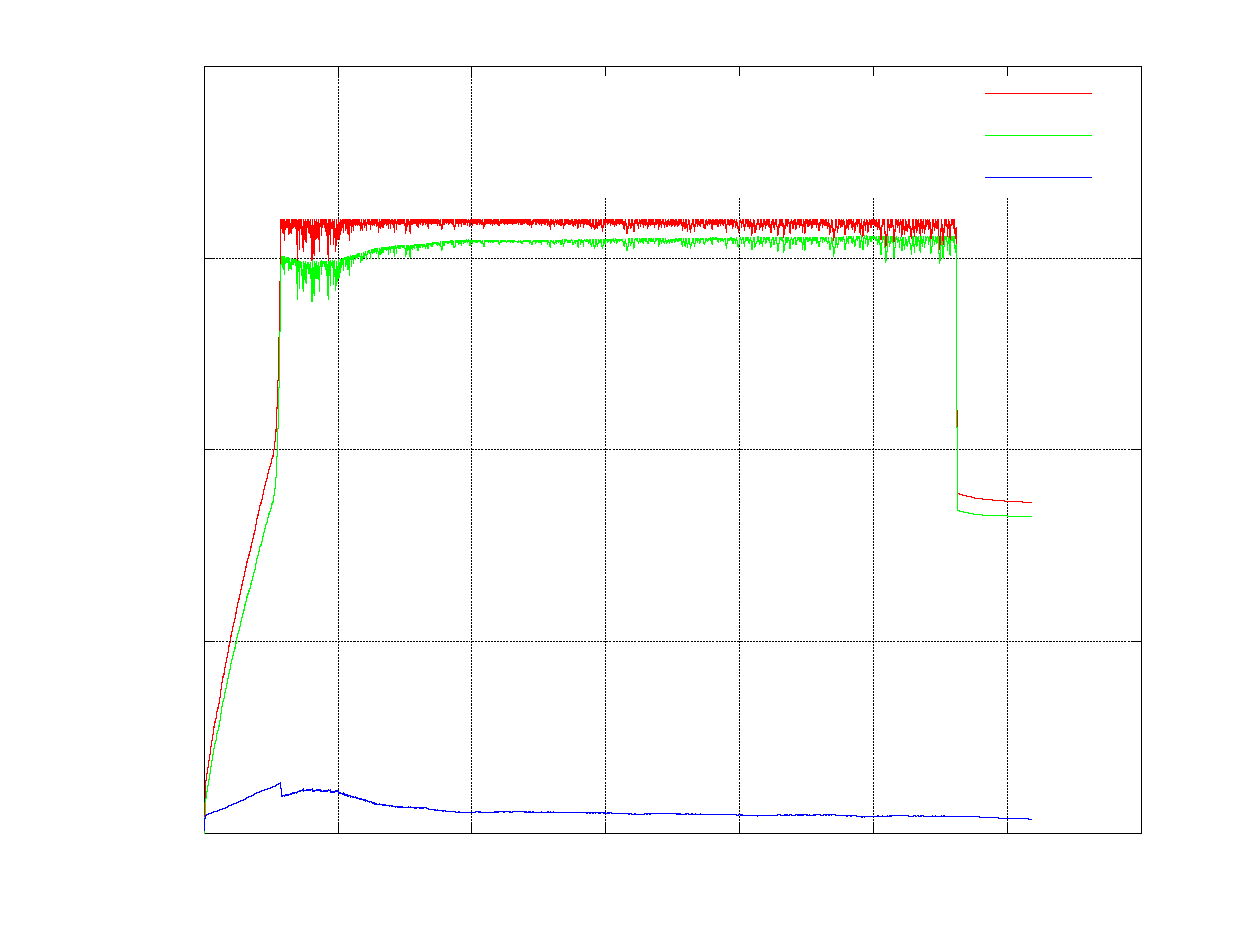
\includegraphics{./images/gmlaslcs0enronFluctuations.eps}}%
    \gplfronttext
  \end{picture}%
\endgroup
}
  \put(-465,115){\rotatebox{90}{Αριθμός μικρο-κανόνων}}
  \put(-380,-20){\rotatebox{0}{Αριθμός δειγμάτων που έχουν παρουσιαστεί στο ΜαΣΤ}}
  \caption{Διακυμάνσεις του αριθμού των κανόνων του πληθυσμού $[P]$ και συμπίεση των χρήσιμων κανόνων του λόγω της υπέρμετρης δημιουργίας κανόνων μηδενικής κάλυψης στον GMl-ASLCS$_{\:0}$.}
  \label{fig:enronFluctuations}
\end{figure}


Στο γράφημα παρατηρούμε:

\begin{enumerate}
\item τις διακυμάνσεις του συνολικού αριθμού μικρο-κανόνων του πληθυσμού, που φτάνει να χάνει μέχρι και $1000$ κανόνες μηδενικής κάλυψης σε ορισμένα χρονικά σημεία, και τη μείωση στο μισό του αριθμού των προκαθορισμένων κανόνων του πληθυσμού προς το τέλος της εκπαιδευτικής διαδικασίας,
\item το βαθμό συμπίεσης που υφίσταται ο πληθυσμός των χρήσιμων κανόνων, λόγω της υπέρ-παραγωγής κανόνων μηδενικής κάλυψης και της αδυναμίας του συστήματος να τους εντοπίσει και να τους αφαιρέσει έγκαιρα, και
\item το γεγονός ότι ο τελικός πληθυσμός κανόνων δεν αποτελείται αμιγώς από κανόνες μη μηδενικής κάλυψης, λόγω της στοχαστικής φύσης της διαγραφής κανόνων μηδενικής κάλυψης και της σχεδιαστικής συνθήκης που επιβάλει ότι σε ένα κανόνα μηδενικής κάλυψης πρέπει να έχει παρουσιαστεί ακέραιο πολλαπλάσιο του αριθμού δειγμάτων $\abs{D}$ τη στιγμή επιλογής κανόνων προς διαγραφή, ώστε να αφαιρεθεί από τον πληθυσμό.
\end{enumerate}



Μία λύση, βεβαίως, θα ήταν να αυξήσουμε το όριο του πληθυσμού σε σημείο τέτοιο ώστε οι πραγματικοί κανόνες του πληθυσμού να φτάσουν τον αριθμό των εξαρχής επιθυμητών κανόνων. Κάτι τέτοιο όμως θα αποτελούσε ημίμετρο, καθώς δεν θα ήρε την απροσδιοριστία για το πραγματικό μέγεθος του πληθυσμού που απαιτεί το πρόβλημα και θα αύξανε κατά πολύ το χρόνο εκπαίδευσης.

\begin{figure}[h!] 
\centering
  \scalebox{0.7}{\Large% GNUPLOT: LaTeX picture with Postscript
\begingroup
  \makeatletter
  \providecommand\color[2][]{%
    \GenericError{(gnuplot) \space\space\space\@spaces}{%
      Package color not loaded in conjunction with
      terminal option `colourtext'%
    }{See the gnuplot documentation for explanation.%
    }{Either use 'blacktext' in gnuplot or load the package
      color.sty in LaTeX.}%
    \renewcommand\color[2][]{}%
  }%
  \providecommand\includegraphics[2][]{%
    \GenericError{(gnuplot) \space\space\space\@spaces}{%
      Package graphicx or graphics not loaded%
    }{See the gnuplot documentation for explanation.%
    }{The gnuplot epslatex terminal needs graphicx.sty or graphics.sty.}%
    \renewcommand\includegraphics[2][]{}%
  }%
  \providecommand\rotatebox[2]{#2}%
  \@ifundefined{ifGPcolor}{%
    \newif\ifGPcolor
    \GPcolorfalse
  }{}%
  \@ifundefined{ifGPblacktext}{%
    \newif\ifGPblacktext
    \GPblacktexttrue
  }{}%
  % define a \g@addto@macro without @ in the name:
  \let\gplgaddtomacro\g@addto@macro
  % define empty templates for all commands taking text:
  \gdef\gplbacktext{}%
  \gdef\gplfronttext{}%
  \makeatother
  \ifGPblacktext
    % no textcolor at all
    \def\colorrgb#1{}%
    \def\colorgray#1{}%
  \else
    % gray or color?
    \ifGPcolor
      \def\colorrgb#1{\color[rgb]{#1}}%
      \def\colorgray#1{\color[gray]{#1}}%
      \expandafter\def\csname LTw\endcsname{\color{white}}%
      \expandafter\def\csname LTb\endcsname{\color{black}}%
      \expandafter\def\csname LTa\endcsname{\color{black}}%
      \expandafter\def\csname LT0\endcsname{\color[rgb]{1,0,0}}%
      \expandafter\def\csname LT1\endcsname{\color[rgb]{0,1,0}}%
      \expandafter\def\csname LT2\endcsname{\color[rgb]{0,0,1}}%
      \expandafter\def\csname LT3\endcsname{\color[rgb]{1,0,1}}%
      \expandafter\def\csname LT4\endcsname{\color[rgb]{0,1,1}}%
      \expandafter\def\csname LT5\endcsname{\color[rgb]{1,1,0}}%
      \expandafter\def\csname LT6\endcsname{\color[rgb]{0,0,0}}%
      \expandafter\def\csname LT7\endcsname{\color[rgb]{1,0.3,0}}%
      \expandafter\def\csname LT8\endcsname{\color[rgb]{0.5,0.5,0.5}}%
    \else
      % gray
      \def\colorrgb#1{\color{black}}%
      \def\colorgray#1{\color[gray]{#1}}%
      \expandafter\def\csname LTw\endcsname{\color{white}}%
      \expandafter\def\csname LTb\endcsname{\color{black}}%
      \expandafter\def\csname LTa\endcsname{\color{black}}%
      \expandafter\def\csname LT0\endcsname{\color{black}}%
      \expandafter\def\csname LT1\endcsname{\color{black}}%
      \expandafter\def\csname LT2\endcsname{\color{black}}%
      \expandafter\def\csname LT3\endcsname{\color{black}}%
      \expandafter\def\csname LT4\endcsname{\color{black}}%
      \expandafter\def\csname LT5\endcsname{\color{black}}%
      \expandafter\def\csname LT6\endcsname{\color{black}}%
      \expandafter\def\csname LT7\endcsname{\color{black}}%
      \expandafter\def\csname LT8\endcsname{\color{black}}%
    \fi
  \fi
  \setlength{\unitlength}{0.0500bp}%
  \begin{picture}(11520.00,8640.00)%
    \gplgaddtomacro\gplbacktext{%
      \colorrgb{0.00,0.00,0.00}%
      \put(780,400){\makebox(0,0)[r]{\strut{}}}%
      \colorrgb{0.00,0.00,0.00}%
      \put(780,2400){\makebox(0,0)[r]{\strut{}$5 \cdot 10^{3}$}}%
      \colorrgb{0.00,0.00,0.00}%
      \put(780,4400){\makebox(0,0)[r]{\strut{}$10 \cdot 10^{3}$}}%
      \colorrgb{0.00,0.00,0.00}%
      \put(780,6399){\makebox(0,0)[r]{\strut{}$15 \cdot 10^{3}$}}%
      \colorrgb{0.00,0.00,0.00}%
      \put(780,8399){\makebox(0,0)[r]{\strut{}$20 \cdot 10^{3}$}}%
      \colorrgb{0.00,0.00,0.00}%
      \put(900,200){\makebox(0,0){\strut{}$0$}}%
      \colorrgb{0.00,0.00,0.00}%
      \put(2366,0){\makebox(0,0){\strut{}$1 \cdot 10^{5}$}}%
      \colorrgb{0.00,0.00,0.00}%
      \put(3831,0){\makebox(0,0){\strut{}$2 \cdot 10^{5}$}}%
      \colorrgb{0.00,0.00,0.00}%
      \put(5297,0){\makebox(0,0){\strut{}$3 \cdot 10^{5}$}}%
      \colorrgb{0.00,0.00,0.00}%
      \put(6762,0){\makebox(0,0){\strut{}$4 \cdot 10^{5}$}}%
      \colorrgb{0.00,0.00,0.00}%
      \put(8228,0){\makebox(0,0){\strut{}$5 \cdot 10^{5}$}}%
      \colorrgb{0.00,0.00,0.00}%
      \put(9693,0){\makebox(0,0){\strut{}$6 \cdot 10^{5}$}}%
      \colorrgb{0.00,0.00,0.00}%
      \put(11159,0){\makebox(0,0){\strut{}$7 \cdot 10^{5}$}}%
    }%
    \gplgaddtomacro\gplfronttext{%
    }%
    \gplbacktext
    \put(0,0){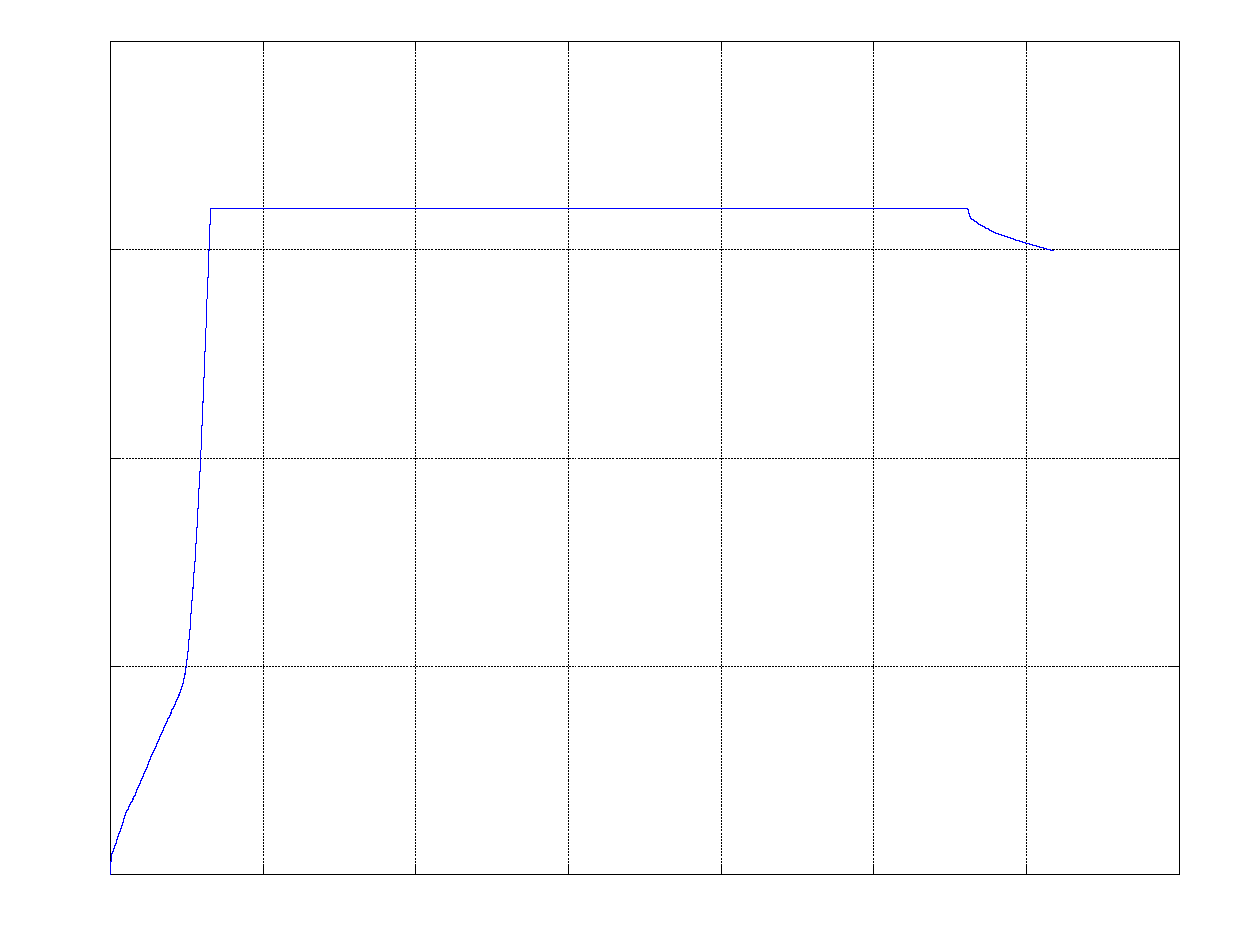
\includegraphics{./images/enronZeroCoveragePrevention.eps}}%
    \gplfronttext
  \end{picture}%
\endgroup
}
  \put(-440,100){\rotatebox{90}{Αριθμός μικρο-κανόνων}}
  \put(-360,-20){\rotatebox{0}{Αριθμός δειγμάτων που έχουν παρουσιαστεί στο ΜαΣΤ}}
  \caption{Ομαλοποίηση του αριθμού των κανόνων του πληθυσμού $[P]$, μέσω της αποφυγής πρόσθεσης κανόνων μηδενικής κάλυψης στον πληθυσμό, στον GMl-ASLCS.}
  \label{fig:enronZeroCoveragePrevention}
\end{figure}

Αντί αυτού, η προσέγγισή μας στα πλαίσια του GMl-ASLCS αντιμετωπίζει το πρόβλημα στη ρίζα του. Κάθε απόγονος, προτού εισαχθεί στον πληθυσμό, ελέγχεται, όπως προαναφέραμε, ως προς την κάλυψη δειγμάτων του συνόλου δεδομένων. Στην περίπτωση μηδενικής κάλυψης ο κανόνας δεν εισάγεται στον πληθυσμό και η εκτέλεση του αλγορίθμου συνεχίζει κανονικά. Με αυτόν τον τρόπο επιτυγχάνεται: 

\begin{itemize}
\item η άρση της απροσδιοριστίας για την κατάσταση του συστήματος, ώστε να καταστεί περισσότερο ελέγξιμο, βοηθώντας στην κατανόηση και μελέτη των λειτουργιών του, και καθιστώντας ευκολότερη τη ρύθμιση παραμέτρων που θα οδηγήσουν σε ορθές λύσεις μέσω του ακριβέστερου προσδιορισμού των παραμέτρων του ΜαΣΤ,

\item η μείωση του συνολικού αριθμού των κανόνων που απαιτούνται για την επίλυση ενός συγκεκριμένου προβλήματος για την εξαγωγή ίδιων αποτελεσμάτων, σε σχέση με την προηγούμενη προσέγγιση του GMl-ASLCS$_{\:0}$ (σε στοχαστικά πλαίσια), και

\item η μείωση του χρόνου εκπαίδευσης για τον ίδιο αριθμό συνολικών μικρο-κανόνων, σε σχέση με τον GMl-ASLCS$_{\:0}$, ανάλογα με το βαθμό φορτικότητας του φαινομένου μηδενικής κάλυψης (όσο μεγαλύτερος ο ρυθμός παραγωγής κανόνων μηδενικής κάλυψης, τόσο μεγαλύτερη και η μείωση του χρόνου χρόνου εκπαίδευσης) και αντιστρόφως ανάλογα με το μέγεθος του συνόλου εκπαίδευσης. 

Με την απαγόρευση εισαγωγής κανόνων μηδενικής κάλυψης στον πληθυσμό, πρέπει να γίνει έλεγχος κάλυψης $\abs{D}$ δειγμάτων για τους κανόνες μηδενικής κάλυψης και ενός απροσδιόριστου αριθμού δειγμάτων $instancesChecked \leq \abs{D}$ για αυτούς που είναι μη μηδενικής κάλυψης, μετά τη δημιουργία τους από τον ΓΑ. Ενδεικτικά, στο πρόβλημα $enron$, για άνω όριο συνολικών μικρο-κανόνων ίσο με $16000$, ο χρόνος εκπαίδευσης του GMl-ASLCS είναι λίγα λεπτά χαμηλότερος από αυτόν του GMl-ASLCS$_{\:0}$, που είναι είναι τρεις ώρες\footnote{Ο χρόνος εκπαίδευσης αυξάνει εκθετικά με την αύξηση του μεγέθους του πληθυσμού.}. 
\end{itemize}



Στο γράφημα του Σχήματος \ref{fig:enronZeroCoveragePrevention} φαίνεται η ομαλοποίηση του αριθμού των μικρο-κανόνων του πληθυσμού, λόγω της αποφυγής πρόσθεσης κανόνων μηδενικής κάλυψης στον πληθυσμό, και η ταύτισή του με τον αριθμό συνολικών μικρο-κανόνων που έχει τεθεί εκ των προτέρων. Η πτώση του παραπάνω αριθμού στο τέλος της εκπαίδευσης εξηγείται στην Παρ. \ref{subsec:controlInM}. 






\subsection{Αφομοίωση-Υπαγωγή Απογόνων}
\label{subsec:subsumptionAndInsertion}
Οι κανόνες που περνούν τον έλεγχο μηδενικής κάλυψης (γραμμές $18$, $19$ της συνάρτησης $evolve$ στον Αλγ. \ref{alg:gmlaslcsGA}) είναι πλέον έτοιμοι προς εισαγωγή στον πληθυσμό $[P]$. Η εισαγωγή στον πληθυσμό, όμως, δε σημαίνει απαραίτητα την αυτοτελή πρόσθεση του κανόνα σε αυτόν. Κάθε απόγονος, όπως περιγράφεται από τη συνάρτηση $checkForSubsumption()$ του Αλγ. \ref{alg:gmlaslcsGAcont}, ελέγχεται πρώτα για \emph{υπαγωγή} από τους γονείς του και ύστερα, σε περίπτωση αποτυχίας, από όλο τον πληθυσμό. Εάν κανένας κανόνας του πληθυσμού δεν πληροί τις προϋποθέσεις για να αφομοιώσει τον απόγονο που παρήχθη, αυτός εισάγεται ως αυτοτελής κανόνας. Τα σύνολα $\textbf{S}$ και $\overline{\textbf{S}}$ στον Αλγ. \ref{alg:gmlaslcsGA} περιέχουν τους απογόνους που θα αφομοιωθούν εν τέλει από κανόνες του πληθυσμού και τους κανόνες που θα εισαχθούν ως αυτοτελείς κανόνες, αντίστοιχα.


\begin{algorithm}
	%\ContinuedFloat
 	\caption{Η λειτουργία αφομοίωσης-υπαγωγής στον GMl-ASLCS}
	\label{alg:gmlaslcsGAcont}
 
  	\begin{algorithmic}[1]
  		\STATE \textbf{\textsc{checkForSubsumption}}($offspring, parents, \textbf{P}, \textbf{S}, \overline{\textbf{S}}$)
  		  	\IF{$(parentA.isEligibleToSubsume(offspring) \: AND \newline parentB.isEligibleToSubsume(offspring))$}

  			\STATE $subsumer \gets fittestAndMostExperienced(parents)$
  			\STATE $\textbf{S}.insert(offspring)$
  			\STATE $return$
		\ELSE
			\IF{$parentA.isEligibleToSubsume(offspring)$}
				\STATE $subsumer \gets parentA$
				\STATE $\textbf{S}.insert(offspring)$
				\STATE $return$
			\ENDIF 
			\IF{$parentB.isEligibleToSubsume(offspring)$}
				\STATE $subsumer \gets parentB$
				\STATE $\textbf{S}.insert(offspring)$
				\STATE $return$
    		\ENDIF
    		
    		\FOR {\textbf{each} $rule \in \textbf{P}$}
    			\STATE $candidateSubsumers \gets rule.isEligibleToSubsume(offspring)$
    		\ENDFOR 
    		\STATE $subsumer \gets fittestAndMostExperienced(candidateSubsumers)$
    		\IF {$subsumer \: found$}
    			\STATE $\textbf{S}.insert(offspring)$
    		\ELSE
    			\STATE $\overline{\textbf{S}}.insert(offspring)$	
    		\ENDIF	
    			
  		\ENDIF

     \end{algorithmic}
\end{algorithm} 

Αναγκαίες συνθήκες ώστε ένας κανόνας $r_{s}$ να αφομοιώσει έναν κανόνα $r$ είναι:
\begin{itemize}
\item Το τμήμα συνθήκης του $r_{s}$ να είναι το ίδιο γενικό ή γενικότερο από του $r$
\item Το τμήμα απόφασης του $r_{s}$ να είναι το ίδιο ειδικό ή ειδικότερο από του $r$
\item Η εμπειρία του $r_{s}$ να ξεπερνάει ένα κατώφλι $\theta_{sub}$
\end{itemize}
   		
Όσον αφορά στην αφομοίωση των απογόνων από τους γονείς τους, ένας απόγονος θα αφομοιωθεί από τον καταλληλότερο γονέα που πληροί τις παραπάνω συνθήκες και, σε περίπτωση ίσης καταλληλότητας, από αυτόν με τη μεγαλύτερη εμπειρία. Αν δεν ικανοποιούνται οι παραπάνω τρεις συνθήκες για τους δύο γονείς, η απόφαση υπαγωγής μεταφέρεται στον πληθυσμό. Εκεί, προτεραιότητα έχουν οι κανόνες με γενικότερο τμήμα συνθήκης και τη μεγαλύτερη καταλληλότητα, καταλήγοντας σε αυτούς με το ίδιο μέγεθος κάλυψης, με την καταλληλότητα των κανόνων να παίζει τον καθοριστικό ρόλο, όπως και πριν. Στην περίπτωση που υπάρχουν παραπάνω του ενός κανόνες, αυτός που θα αφομοιώσει τον απόγονο θα είναι αυτός που δημιουργήθηκε τελευταίος χρονικά. Οι κανόνες που έχουν προκύψει μέσω του Τμήματος Κάλυψης δεν ελέγχονται για υπαγωγή και εισέρχονται αυτοτελώς στον πληθυσμό του GMl-ASLCS.

Σε κάθε περίπτωση, αφού βρεθεί ο κανόνας $r_{s}$ που θα αφομοιώσει τον απόγονο $r$, ο $r$ δεν εισάγεται στον πληθυσμό και η πληθικότητα του $r_{s}$ αυξάνει κατά ένα. Σε αντίθετη περίπτωση, ο $r$ εισάγεται ως αυτόνομος κανόνας στον πληθυσμό $[P]$, με αρχικές συνθήκες $(tp, msa, cs, fitness) = (0,0,1,1)$.

Η λειτουργία της αφομοίωσης αποτρέπει τη συσσώρευση υπέρ-ειδικών κανόνων, λειτουργώντας, έτσι, ενισχυτικά προς τη διατήρηση κανόνων σε ένα επίπεδο γενικότητας. Ακριβώς για τον ίδιο λόγο, όμως, μπορεί να δυσχεραίνει την εξερεύνηση του χώρου αναζήτησης, αποτρέποντας υπέρ-ειδικούς κανόνες, που κωδικοποιούν ένα μέρος της λύσης και λειτουργούν βοηθητικά προς αυτή, από το να συμμετάσχουν στον πληθυσμό.


\subsection{Διαδικασία Εισαγωγής Απογόνων στον Πληθυσμό}
Για ένα πρόβλημα πολυκατηγορικής ταξινόμησης με $\abs{L}$ ετικέτες, η εισαγωγή ενός δείγματος για εκπαίδευση στο ΜαΣΤ έχει ως αποτέλεσμα το σχηματισμό $\abs{L}$ Correct Sets, από το καθένα από τα οποία είτε θα προκύψουν ακριβώς δύο απόγονοι, ή κανένας. Συνεπώς, συνολικά, η εισαγωγή ενός δείγματος εκπαίδευσης έχει ως αποτέλεσμα την παραγωγή $k$ απογόνων, όπου $k=2 \cdot m$ με $m \in \mathbb{N}$ και $m \in [0,\abs{L}]$. Ενώ στον GMl-ASLCS$_{\:0}$ η διαδικασία εισαγωγής ενσωματώνει κάθε κανόνα στον πληθυσμό απευθείας μετά την παραγωγή του, ο GMl-ASLCS χρησιμοποιεί ένα σχήμα μαζικής εισαγωγής των απογόνων που παράγονται συνολικά από την είσοδο ενός δείγματος στο ΜαΣΤ.

Αφενός, αυτό γίνεται για λόγους οικονομίας χρόνου και υπολογισμών. Στην πρώτη περίπτωση, για τη συνολική εισαγωγή $k$ απογόνων στον πληθυσμό $[P]$, εάν έχει ξεπεραστεί ο μέγιστος αριθμός κανόνων που έχει θέσει ο χρήστης, σε κάθε γενετικό συμβάν πρέπει να υπολογιστούν 

\begin{equation}
k \cdot (\abs{P} + 1)
\end{equation}
\\
πιθανότητες διαγραφής, ενώ στη δεύτερη 

\begin{equation}
\abs{P} + k
\end{equation}
\\
Αφετέρου, τα διενεργηθέντα πειράματα σε τεχνητά και πραγματικά σύνολα δεδομένων δείχνουν πως η δεύτερη μέθοδος εισαγωγής κανόνων στον πληθυσμό επιδεικνύει συνολικά καλύτερες επιδόσεις από την πρώτη.

Συνολικά, όπως φαίνεται και στον Αλγ. \ref{alg:gmlaslcsTrainCycle}, η συνάρτηση  $controlPopulation$ καλείται μία φορά ανά δείγμα σε περίπτωση που ο αριθμός των μικρο-κανόνων έχει  ξεπεράσει το όριο $maximumPopulationSize$ που έχουμε θέσει (Αλγ. \ref{alg:gmlaslcsTrainCycle}, γρ. $27$, $28$), αντί για $k$ φορές (Αλγ. \ref{alg:gmlaslcs0Update}, γρ. $20$, $21$). Στους αλγορίθμους \ref{alg:gmlaslcsTrainCycle} και \ref{alg:gmlaslcsGAcont}, τα σύνολα κανόνων $\textbf{S}$ και $\overline{\textbf{S}}$ υποδηλώνουν το σύνολο στο οποίο τοποθετούνται οι κανόνες που προορίζονται προς αφομοίωση και αυτό στο οποίο τοποθετούνται κανόνες που θα εισαχθούν στον πληθυσμό ως αυτόνομοι, αντίστοιχα,
με $\abs{\textbf{S}}+\abs{\overline{\textbf{S}}} = k$.


\subsection{Λειτουργία Διαγραφής}
\label{subsec:gmlaslcsDeletion}
Όπως προαναφέραμε, η λειτουργία διαγραφής ενεργοποιείται κάθε φορά που είναι αληθής η συνθήκη
\begin{equation}
\label{eq:deletionRequirement}
\sum microClassifiers > maximumPopulationSize
\end{equation}
\\
όπου $maximumPopulationSize$ το άνω όριο για το συνολικό αριθμό μικρο-κανόνων που διατηρεί το ΜαΣΤ στον πληθυσμό $[P]$. Μετά από κάθε εισαγωγή απογόνων στον πληθυσμό, ελέγχεται η ισχύς της (\ref{eq:deletionRequirement}) και, όταν βρεθεί αληθής, επιλέγονται για διαγραφή τόσοι κανόνες όση η διαφορά

 
\begin{equation}
\sum microClassifiers - maximumPopulationSize
\end{equation}
\\
χρησιμοποιώντας επιλογή ρουλέτας. 

Σε κάθε κανόνα $i$ του πληθυσμού $[P]$ ανατίθεται μία πιθανότητα επιλογής $P(i)$:

\begin{equation}
\label{eq:deletionRouletteGMlASLCS}
P(i) = \frac{num(i) \cdot d(i)}{\sum\limits_{j=1}^n \big(num(j) \cdot d(j)\big)}
\end{equation}
\\
με $d(i)$:


\begin{equation}
\label{eq:deletionFormula}
d(i) = \left\{
\begin{array}{ c l }
\displaystyle e^{\dfrac{1}{fitness(i)}}, & experience(i) < \theta_{del} 
\\
\\

\displaystyle \dfrac{e^{\displaystyle cs(i)-1}}{fitness(i)}, & $αλλού$
\end{array}
\right.
\end{equation}
\\
Η Εξ. \ref{eq:deletionFormula} δείχνει ότι αποφεύγουμε συνολικά τη χρήση της μέσης καταλληλότητας του πληθυσμού $F_{P}$, καθώς και τη χρήση του $cs$ για τους κανόνες των οποίων η εμπειρία είναι μικρή, δηλαδή έχουν συμμετάσχει σε λιγότερα από $\theta_{del}$ Match Sets. Η χρήση της μέσης καταλληλότητας $F_{P}$ βρέθηκε πειραματικά ότι δεν έχει κάποια βοηθητική δράση στις επιδόσεις του GMl-ASLCS (συγκεκριμένα για τις μετρικές της Ακρίβειας και της Μέσης Κάλυψης δειγμάτων από τους κανόνες του), στο υφιστάμενο πλαίσιο διαγραφής, ενώ ο υπολογισμός της εισάγει πρόσθετη χρονική πολυπλοκότητα. Όσον αφορά στην εκτίμηση του μεγέθους των Correct Sets $cs$ στα οποία συμμετέχει ένας κανόνας, αυτή δεν χρησιμοποιείται για τους κανόνες με $experience < \theta_{del}$, λόγω της υπερεκτίμησης του πραγματικού μεγέθους των Correct Sets στα οποία συμμετέχουν, η οποία μπορεί να οδηγήσει σε μη αξιόπιστες διαγραφές. 

Το γράφημα του Σχήματος \ref{fig:emotionsNsPlusCov} παριστά με μπλε χρώμα το μέσο όρο των $cs$ των κανόνων του πληθυσμού και με κόκκινο το μέσο αριθμό καλυπτόμενων δειγμάτων από τον πληθυσμό $[P]$ των κανόνων, για το πρόβλημα $music$. Ο κατακόρυφος άξονας συμβολίζει το μέσο αριθμό κανόνων των Correct Sets για την καμπύλη με μπλε χρώμα και το μέσο αριθμό δειγμάτων που καλύπτουν οι κανόνες του πληθυσμού για την καμπύλη με κόκκινο χρώμα. Παρατηρούμε δύο διακριτά διαστήματα: το πρώτο, όπου το $\overline{cs}$ αυξάνει γραμμικά, και το δεύτερο, στο οποίο φθίνει εκθετικά.

\begin{figure}[h!] 
\centering
  \scalebox{0.7}{\Large% GNUPLOT: LaTeX picture with Postscript
\begingroup
  \makeatletter
  \providecommand\color[2][]{%
    \GenericError{(gnuplot) \space\space\space\@spaces}{%
      Package color not loaded in conjunction with
      terminal option `colourtext'%
    }{See the gnuplot documentation for explanation.%
    }{Either use 'blacktext' in gnuplot or load the package
      color.sty in LaTeX.}%
    \renewcommand\color[2][]{}%
  }%
  \providecommand\includegraphics[2][]{%
    \GenericError{(gnuplot) \space\space\space\@spaces}{%
      Package graphicx or graphics not loaded%
    }{See the gnuplot documentation for explanation.%
    }{The gnuplot epslatex terminal needs graphicx.sty or graphics.sty.}%
    \renewcommand\includegraphics[2][]{}%
  }%
  \providecommand\rotatebox[2]{#2}%
  \@ifundefined{ifGPcolor}{%
    \newif\ifGPcolor
    \GPcolorfalse
  }{}%
  \@ifundefined{ifGPblacktext}{%
    \newif\ifGPblacktext
    \GPblacktexttrue
  }{}%
  % define a \g@addto@macro without @ in the name:
  \let\gplgaddtomacro\g@addto@macro
  % define empty templates for all commands taking text:
  \gdef\gplbacktext{}%
  \gdef\gplfronttext{}%
  \makeatother
  \ifGPblacktext
    % no textcolor at all
    \def\colorrgb#1{}%
    \def\colorgray#1{}%
  \else
    % gray or color?
    \ifGPcolor
      \def\colorrgb#1{\color[rgb]{#1}}%
      \def\colorgray#1{\color[gray]{#1}}%
      \expandafter\def\csname LTw\endcsname{\color{white}}%
      \expandafter\def\csname LTb\endcsname{\color{black}}%
      \expandafter\def\csname LTa\endcsname{\color{black}}%
      \expandafter\def\csname LT0\endcsname{\color[rgb]{1,0,0}}%
      \expandafter\def\csname LT1\endcsname{\color[rgb]{0,1,0}}%
      \expandafter\def\csname LT2\endcsname{\color[rgb]{0,0,1}}%
      \expandafter\def\csname LT3\endcsname{\color[rgb]{1,0,1}}%
      \expandafter\def\csname LT4\endcsname{\color[rgb]{0,1,1}}%
      \expandafter\def\csname LT5\endcsname{\color[rgb]{1,1,0}}%
      \expandafter\def\csname LT6\endcsname{\color[rgb]{0,0,0}}%
      \expandafter\def\csname LT7\endcsname{\color[rgb]{1,0.3,0}}%
      \expandafter\def\csname LT8\endcsname{\color[rgb]{0.5,0.5,0.5}}%
    \else
      % gray
      \def\colorrgb#1{\color{black}}%
      \def\colorgray#1{\color[gray]{#1}}%
      \expandafter\def\csname LTw\endcsname{\color{white}}%
      \expandafter\def\csname LTb\endcsname{\color{black}}%
      \expandafter\def\csname LTa\endcsname{\color{black}}%
      \expandafter\def\csname LT0\endcsname{\color{black}}%
      \expandafter\def\csname LT1\endcsname{\color{black}}%
      \expandafter\def\csname LT2\endcsname{\color{black}}%
      \expandafter\def\csname LT3\endcsname{\color{black}}%
      \expandafter\def\csname LT4\endcsname{\color{black}}%
      \expandafter\def\csname LT5\endcsname{\color{black}}%
      \expandafter\def\csname LT6\endcsname{\color{black}}%
      \expandafter\def\csname LT7\endcsname{\color{black}}%
      \expandafter\def\csname LT8\endcsname{\color{black}}%
    \fi
  \fi
  \setlength{\unitlength}{0.0500bp}%
  \begin{picture}(11520.00,8640.00)%
    \gplgaddtomacro\gplbacktext{%
      \colorrgb{0.00,0.00,0.00}%
      \put(1080,800){\makebox(0,0)[r]{\strut{}$0$}}%
      \colorrgb{0.00,0.00,0.00}%
      \put(1080,1781){\makebox(0,0)[r]{\strut{}$20$}}%
      \colorrgb{0.00,0.00,0.00}%
      \put(1080,2762){\makebox(0,0)[r]{\strut{}$40$}}%
      \colorrgb{0.00,0.00,0.00}%
      \put(1080,3744){\makebox(0,0)[r]{\strut{}$60$}}%
      \colorrgb{0.00,0.00,0.00}%
      \put(1080,4725){\makebox(0,0)[r]{\strut{}$80$}}%
      \colorrgb{0.00,0.00,0.00}%
      \put(1080,5706){\makebox(0,0)[r]{\strut{}$100$}}%
      \colorrgb{0.00,0.00,0.00}%
      \put(1080,6687){\makebox(0,0)[r]{\strut{}$120$}}%
      \colorrgb{0.00,0.00,0.00}%
      \put(1080,7668){\makebox(0,0)[r]{\strut{}$140$}}%
      \colorrgb{0.00,0.00,0.00}%
      \put(1320,400){\makebox(0,0){\strut{}$0$}}%
      \colorrgb{0.00,0.00,0.00}%
      \put(2900,400){\makebox(0,0){\strut{}$0.5 \cdot 10^{5}$}}%
      \colorrgb{0.00,0.00,0.00}%
      \put(4480,400){\makebox(0,0){\strut{}$1 \cdot 10^{5}$}}%
      \colorrgb{0.00,0.00,0.00}%
      \put(6060,400){\makebox(0,0){\strut{}$1.5 \cdot 10^{5}$}}%
      \colorrgb{0.00,0.00,0.00}%
      \put(7639,400){\makebox(0,0){\strut{}$2 \cdot 10^{5}$}}%
      \colorrgb{0.00,0.00,0.00}%
      \put(9219,400){\makebox(0,0){\strut{}$2.5 \cdot 10^{5}$}}%
      \colorrgb{0.00,0.00,0.00}%
      \put(10799,400){\makebox(0,0){\strut{}$3 \cdot 10^{5}$}}%
    }%
    \gplgaddtomacro\gplfronttext{%
      \csname LTb\endcsname%
      \put(9056,7896){\makebox(0,0)[r]{\strut{}$\overline{cs}$}}%
      \csname LTb\endcsname%
      \put(9056,7496){\makebox(0,0)[r]{\strut{}$\overline{instances}$}}%
    }%
    \gplbacktext
    \put(0,0){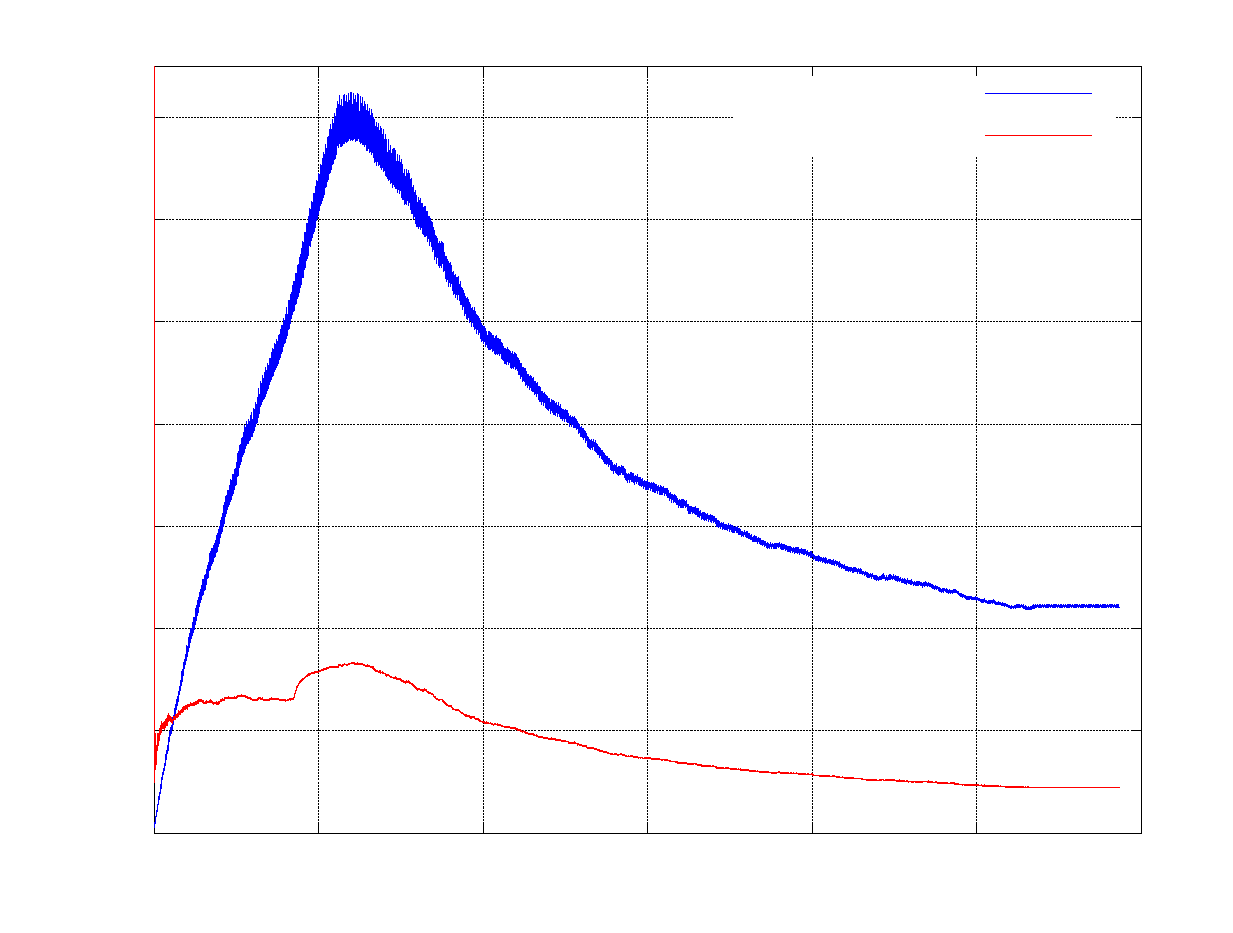
\includegraphics{./images/emotionsNsPlusCov.eps}}%
    \gplfronttext
  \end{picture}%
\endgroup
}
  \put(-360,-20){\rotatebox{0}{Αριθμός δειγμάτων που έχουν παρουσιαστεί στον πληθυσμό}}
   \put(-440,30){\rotatebox{90}{\parbox{9cm}{Μέσος αριθμός κανόνων των Correct Sets και \\ Μέσος αριθμός δειγμάτων που καλύπτουν οι\\ κανόνες του πληθυσμού}}}

  \caption{Καμπύλες εξέλιξης του μέσου $cs$ και του μέσου αριθμού καλυπτόμενων δειγμάτων από τους κανόνες του πληθυσμού στο πρόβλημα music.}
  \label{fig:emotionsNsPlusCov}
\end{figure}


Στο πρώτο διάστημα, ο αριθμός των κανόνων αυξάνει, χωρίς να έχει φτάσει το άνω όριό του και, άρα, χωρίς να έχουν γίνει διαγραφές κανόνων. Όσο αυξάνει ο αριθμός των κανόνων, αυξάνει και ο αριθμός των κανόνων που συμμετέχουν σε Correct Sets, λόγω της αναπαραγωγής κανόνων με βάση τους κανόνες που συμμετέχουν σε αυτά. Έτσι, για κάθε κανόνα, αυξάνει και η εκτίμηση για τον αριθμό κανόνων $cs$ στα Correct Sets που συμμετέχει, αυξάνοντας συνεπώς και το μέσο $cs$ ($\overline{cs}$) των κανόνων του πληθυσμού. Η εκτίμηση $cs$ του μεγέθους των $[C]$ βρίσκεται πάντα χαμηλότερα από το πραγματικό $cs$, όσο αυξάνει το $minCs$, λόγω της σχέσης 

\begin{equation}
\label{eq:csGMlASLCS}
rule.cs \gets rule.cs + \beta \cdot (minCs - rule.cs)
\end{equation}
\\
που χρησιμοποιείται. Μάλιστα, η υποεκτίμηση αυξάνει σε μέγεθος όσο μεγαλύτερες είναι οι διαφορές $minCs - rule.cs$. Στους πίνακες \ref{tbl:csUnderestimation} και \ref{tbl:csOverestimation} παρατίθενται τεχνητά μεγέθη για το ελάχιστο μέγεθος των Correct Sets στα οποία συμμετέχει ένας κανόνας, η πραγματική τιμή του μέσου μεγέθους $cs$, υπολογισμένη ως ο μέσος όρος των $minCs$ και η εκτίμηση για το μέσο $cs$ των κανόνων. Ο αναγνώστης θα παρατηρήσει πως όσο αυξάνει ο αριθμός συμμετοχών ενός κανόνα σε Correct Set, τόσο μικρότερο είναι το σφάλμα για το πραγματικό μέσο μέγεθος των αριθμών των κανόνων των Correct Sets στα οποία αυτός συμμετέχει.

\begin{table}[!htb]
    \begin{minipage}{.5\linewidth}
    	\centering
      	\caption{Υποεκτίμηση \\του πραγματικού $cs$, για $\beta=0.2$, \\πριν την έναρξη των διαγραφών \\με επιλογή ρουλέτας.}
      	\label{tbl:csUnderestimation}
        \begin{tabular}{cc|c}
            \hline \\ [-1.5ex]
    		$min(cs)$ & Πραγματικό $cs$    & $cs$ 
			\\[1ex] \hline
    		20      &	20	&	20   	\\
    		40    	&	30	& 	24 		\\
    		60    	&	40	& 31.2		\\
    		80     	&	50	& 40.96		\\
    		100     &	60	& 52.768   	\\
			\hline
        \end{tabular}
    \end{minipage}%
    \begin{minipage}{.5\linewidth}
      	\centering
      	\caption{Υπερεκτίμηση \\του πραγματικού $cs$, για $\beta=0.2$, \\μετά την έναρξη των διαγραφών \\με επιλογή ρουλέτας.}
      	\label{tbl:csOverestimation}
        \begin{tabular}{cc|c}
			\hline \\ [-1.5ex]
    		$min(cs)$ & Πραγματικό $cs$    & $cs$ 
			\\[1ex] \hline
   			100     &	100	& 100   	\\
   			80    	&	90	& 96 		\\
    		60    	&	80	& 88.8		\\
    		40     	&	70	& 79.04		\\
    		20      &	60	& 67.232  	\\
			\hline
        \end{tabular}
    \end{minipage} 
\end{table}



Το δεύτερο διάστημα, όπου το μέσο $cs$ φθίνει εκθετικά, είναι αυτό στο οποίο διαγράφονται κανόνες. Οι διαγραφές ξεκινούν στο ολικό μέγιστο της καμπύλης του Σχήματος \ref{fig:emotionsNsPlusCov}. Στον Πίνακα \ref{tbl:csOverestimation} βλέπουμε, αντίστοιχα με την υποεκτίμηση που συμβαίνει στο πρώτο διάστημα, την υπερεκτίμηση του μέσου μεγέθους $cs$ των κανόνων του πληθυσμού, για το διάστημα στο οποίο διαγράφονται κανόνες σύμφωνα με την Εξ. \ref{eq:deletionFormula}, στο οποίο παρατηρείται η πτώση του $\overline{cs}$ των κανόνων. Εάν διαγράφαμε κανόνες που είναι σχετικά άπειροι, με $experience < \theta_{del}$, που δημιουργήθηκαν μετά την έναρξη των διαγραφών, έχοντας ως κριτήριο και την εκτίμηση $cs$, τότε, θα στερούσαμε από τον πληθυσμό καινούριους κανόνες οι οποίοι ίσως να ήταν χρήσιμοι αλλά η εκτίμηση του πραγματικού $cs$ τους είναι σαφέστατα μεγαλύτερη από την πραγματική τιμή του. Παράλληλα, δεν θα είχε σταθεροποιηθεί η εκτίμηση ακόμα, τόσο, ώστε να τους ανατεθεί μία ακριβέστερη πιθανότητα διαγραφής. Αν εξετάσουμε το ζήτημα υπό το πρίσμα του δευτέρου μέρους της Εξ. \ref{eq:deletionFormula}, είναι δυνατόν, το μέγεθος $cs$ κανόνων σχετικά νέων στον πληθυσμό, καθώς φθίνει γενικότερα το μέγεθος $cs$ των κανόνων, να είχε τιμή μεγαλύτερη από αυτό κανόνων έμπειρων, που δημιουργήθηκαν πριν την έναρξη των διαγραφών, των οποίων το μέγεθος $cs$ είναι χαμηλότερο λόγω της υποεκτίμησης του πραγματικού $cs$ στο πρώτο διάστημα.

Για αυτό το λόγο, επιλέγουμε να αναθέσουμε σε κανόνες των οποίων η εμπειρία είναι χαμηλότερη από το κατώφλι $\theta_{del}$, μία πιθανότητα διαγραφής που δε χρησιμοποιεί την εκτίμηση $cs$, αλλά είναι αντιστρόφως ανάλογη προς την καταλληλότητά τους και σε εκθετική μορφή, ώστε νέοι κανόνες, χαμηλής καταλληλότητας, να έχουν συγκρίσιμη πιθανότητα διαγραφής ως προς αυτούς που είναι εμπειρότεροι. Θέτοντας μάλιστα το $\theta_{del}$ σε μία τιμή λογική ως προς το μέσο ποσοστό κάλυψης των κανόνων, φροντίζουμε ώστε οι κανόνες που έχουν παραχθεί πρόσφατα σε σχέση με τη στιγμή που τους ανατίθενται πιθανότητες διαγραφής, να έχουν αξιολογηθεί ως προς τα περισσότερα, αν όχι όλα, τα δείγματα που καλύπτουν, έτσι ώστε να έχει σταθεροποιηθεί η καταλληλότητά τους και να μην υπάρχουν κανόνες που αδικούνται από το σχήμα διαγραφής.


Όσον αφορά στο δεύτερο μέρος της Εξ. \ref{eq:deletionFormula}, αυτό βασίζεται, όπως και στις προσεγγίσεις της βιβλιογραφίας, στην εκτίμηση $cs$. Η δική μας προσέγγιση χρησιμοποιεί, ως πρόσθετο βάρος στην πιθανότητα διαγραφής, την καταλληλότητα του κανόνα, αλλά με μικρότερο βαθμό επιρροής σε σχέση με αυτόν του $cs$. Η, σχεδόν αποκλειστική, χρήση του μεγέθους $cs$ οφείλεται σε δύο λόγους: 

\begin{enumerate}
\item Διαγράφοντας έχοντας ως κριτήριο το $cs$,  τείνουν να εξισορροπηθούν σε μέγεθος τα διαφορετικά Correct Sets, κατανέμοντας στο καθένα έναν ίσο αριθμό κανόνων με όλα τα υπόλοιπα \cite{XCS}. Πράγματι, ένας κανόνας έχει μεγαλύτερη πιθανότητα διαγραφής όταν συμμετέχει σε $[C]$ με μεγάλο μέγεθος. Με αυτό τον τρόπο, επαναληπτικά, μειώνονται οι κανόνες που συμμετέχουν σε υπερπληθή $[C]$, εξισορροπώντας τα μεγέθη των διαφόρων Correct Sets.

\item Από τα αποτελέσματα και τις παρατηρήσεις μας, φαίνεται ότι αποτελεί ένα αξιόπιστο κριτήριο διαγραφής. 

Αυτή η εργασία, επιλέγει να χρησιμοποιήσει ως ένα δεύτερο κριτήριο και το μέγεθος της καταλληλότητας, ώστε να διαχωρίζονται καλύτερα κανόνες που συμμετέχουν σε Correct Sets με παρόμοιο μέγεθος, βοηθώντας στην προαγωγή των καταλληλότερων κανόνων. Το ζήτημα της υπερεκτίμησης είναι παρόν και εδώ, αλλά σε μικρότερο βαθμό από ότι για κανόνες με εμπειρία μικρότερη από $\theta_{del}$ και, μάλιστα, με μειούμενη επιρροή όσο μεγαλύτερη είναι η εμπειρία ενός κανόνα. Όσο μεγαλύτερη είναι η εμπειρία του, τόσες περισσότερες φορές έχει εκτιμηθεί η πραγματική τιμή του $cs$, άρα τόσο “μικρότερη" είναι η υπερεκτίμηση για αυτό, όπως φαίνεται και στους Πίνακες \ref{tbl:csUnderestimation} και \ref{tbl:csOverestimation}.
\end{enumerate}

  
Ο αναγνώστης θα παρατηρήσει πως και στα δύο μέρη της Εξ. \ref{eq:deletionFormula} χρησιμοποιούμε ως εκθέτες με βάση $e$ τα κριτήρια στα οποία στηρίζονται οι διαγραφές. Η εκθετική μορφή χρησιμοποιείται ώστε να διαχωρίσει ακριβέστερα και με μεγαλύτερη αποφασιστικότητα κανόνες με μικρές διαφορές (ως προς το μέγεθος $cs$ ή ανάμεσα στην καταλληλότητα και το $cs$), ανάλογα και με το μέγεθος της υπερεκτίμησης για τον κάθε κανόνα με $experience \geq \theta_{del}$.





\section{Συνιστώσα Ενίσχυσης}
Η Συνιστώσα Ενίσχυσης τροποποιείται σημαντικά στον GMl-ASLCS, με δύο σημεία διαφοροποίησης, τα οποία μπορούμε να εντοπίσουμε στον Αλγ. \ref{alg:gmlaslcsTrainCycle}. Η πρώτη διαφοροποίηση βρίσκεται στον έλεγχο και τη λειτουργία της συνάρτησης $controlMatchSet$ (γραμμές 3 και 4, αντίστοιχα, του αλγορίθμου \ref{alg:gmlaslcsTrainCycle}). Η λειτουργία και οι λόγοι για την επινόηση της διαδικασίας που υλοποιείται στη μέθοδο $controlMatchSet$ περιγράφονται στην Παρ. \ref{subsec:controlInM}. Η δεύτερη τροποποίηση παρουσιάζεται στην επόμενη ενότητα και εντοπίζεται στη συνάρτηση $updateFitness$ (γρ. $10$ του Αλγ. \ref{alg:gmlaslcsTrainCycle}). Αφορά στον τρόπο χειρισμού των αδιαφοριών για ετικέτες στο καίριο σημείο της λογικής μεταβολής της καταλληλότητας ενός κανόνα που συμμετέχει σε ένα Match Set, αλλά αδιαφορεί για μία ετικέτα $l$.


\subsection{Ενημέρωση Καταλληλότητας}
\label{subsec:gmlaslcsupdate}
Η ακριβής μεθοδολογία ενημέρωσης των μεταβλητών που σχετίζονται με την καταλληλότητα περιγράφεται από τον Αλγ. \ref{alg:gmlaslcsUpdateFitness}.

\begin{algorithm} 
 \caption{Ενημέρωση της καταλληλότητας στον GMl-ASLCS.}
\label{alg:gmlaslcsUpdateFitness}
 \begin{algorithmic}[1]
  	\STATE \textbf{\textsc{updateFitness}}($rule$)
  	\STATE $rule.exp \gets rule.exp + 1$
  	\FOR {\textbf{each} $l \in L$}
  		\STATE $rule.tp \gets rule.tp + correctness(rule, l)$
  		\STATE $rule.msa \gets rule.msa + msaValue(rule, l)$
  	\ENDFOR
  	\STATE $rule.fitness \gets \Big(\dfrac{rule.tp}{rule.msa}\Big)^{\nu}$

 \end{algorithmic}
\end{algorithm}

Για κάθε κανόνα στο Match Set, εξετάζεται η ικανότητά του για κατηγοριοποίηση του $Instance$ σε κάθε ετικέτα $l$. Επίσης για κάθε ετικέτα, οι ποσότητες $tp$ και $msa$ αυξάνονται κατά ποσό ανάλογο της ικανότητας κατηγοριοποίησης ($correctness$) του κανόνα σε αυτή. Τα μεγέθη $tp$ και $msa$ αναπαριστούν και εδώ τον αριθμό ορθών κατηγοριοποιήσεων ενός κανόνα και τον ολικό αριθμό κατηγοριοποιήσεών του, αντίστοιχα. Λόγω της χρήσης αναπαράστασης ετικετών με αδιαφορίες, όμως, είναι αναγκαίο να εξετάσουμε το μέγεθος της ποσότητας “ανταμοιβής" που θα πρέπει να λάβει ένας κανόνας, σε περίπτωση αδιαφορίας για μία ετικέτα.
Φορμαλιστικά:

\begin{equation}
\label{eq:gmlAslcsOmega}
correctness(rule, l) = \left\{
\begin{array}{ c l }
	\displaystyle 1, & $ εάν ο $ rule $ προβλέπει ορθά την $ l
	\\
	\displaystyle 0, & $ εάν ο $ rule $ προβλέπει λανθασμένα την $ l
	\\
	\displaystyle \omega, & $ εάν ο $ rule $ αδιαφορεί για την $ l
\end{array}
\right.
\end{equation}
\\
Προφανώς, σε περίπτωση ορθής κατηγοριοποίησης το μέγεθος $tp$ θα αυξηθεί κατά ένα, και σε περίπτωση λανθασμένης θα μείνει αμετάβλητο. Στην περίπτωση της αδιαφορίας, όμως, δε θα ήταν σχεδιαστικά και εξελικτικά ορθό να χρησιμοποιήσουμε κάποια από αυτές τις δύο ακραίες τιμές: ο κανόνας δεν κατηγοριοποιεί ούτε ορθά για να λάβει το πλήρες ποσό της ανταμοιβής, ούτε λανθασμένα ώστε να μην λάβει κάποια ανταμοιβή. 

Επιπρόσθετα, η επιζητούμενη ποσότητα θα πρέπει να ιδωθεί και υπό το πρίσμα της έκπτωσης στην καταλληλότητα που προσδίδει η παράμετρος $\nu$. Ακόμα και αν θέταμε την τιμή του $\omega$ στο μέσο όρο των δύο ακραίων τιμών ορθότητας, υποθέτοντας έστω και μία αδιαφορία, η ύψωση στη νιοστή δύναμη\footnote{Η τιμή που χρησιμοποιείται σχεδόν αποκλειστικά στη βιβλιογραφία είναι $\nu=10$.} της ακρίβειας $acc = tp / msa$ θα καθιστούσε τον κανόνα λιγότερο επιλέξιμο πιθανοτικά για αναπαραγωγή και περισσότερο για διαγραφή από όσο του “αξίζει", κάνοντας την προσέγγισή μας πολύ αυστηρή. 

Παράλληλα, ο καθορισμός μίας ορθολογικής τιμής για το $\omega$ θα πρέπει να γίνει σε συνδυασμό με τον καθορισμό της τιμής $\phi$:
\\


\begin{equation}
\label{eq:gmlAslcsPhi}
msaValue(rule, l) = \left\{
\begin{array}{ c l }
	\displaystyle \phi, & $ εάν ο $ rule $ αδιαφορεί για την $ l
	\\
	\displaystyle 1, & $αλλού$
\end{array}
\right.
\end{equation}
\\
Η προσέγγιση που ακολουθείται εν τέλει, θέτει το $\omega=0.9$ και το $\phi=1$. Έτσι, για έναν κανόνα, για κάθε ετικέτα που αδιαφορεί, γίνεται έκπτωση 0.1 από την τιμή της ορθής κατηγοριοποίησης, μεταβάλλοντας την καταλληλότητά του στην:

\begin{equation}
fitness=\Big(\frac{tp + 0.9}{msa + 1}\Big)^{\nu}
\end{equation}










\subsection{Διεύρυνση της Μέσης Κάλυψης}
\label{subsec:controlInM}
Όπως έχει προαναφερθεί, το (κατά το δυνατόν) υψηλό ποσοστό κάλυψης δειγμάτων από τους κανόνες είναι μία από τις προϋποθέσεις για την αποτελεσματικότητα και ακρίβεια πρόβλεψης κάθε Μανθάνοντος Συστήματος Ταξινομητών. Ο GMl-ASLCS$_{\:0}$, παρ' όλα αυτά, εξέλισσε κανόνες των οποίων ο μέσος αριθμός δειγμάτων που κάλυπταν βρίσκονταν σε σχετικά χαμηλά επίπεδα, όπως σημειώνεται και στον Πίνακα \ref{table:gmlaslcs0coverageForgmlaslcs}. Η σχετικότητα έγκειται αφενός στη φύση και τα χαρακτηριστικά ενός δεδομένου προβλήματος, αφετέρου στις παραμέτρους και τις επιμέρους λειτουργίες του ίδιου του ΜαΣΤ. 

\begin{table}[!h]
\begin{center}
\caption{Μέση Κάλυψη δειγμάτων από τους κανόνες, όπως προκύπτει πειραματικά για τον GMl-ASLCS$_{\:0}$, για τα έξι σύνολα πολυκατηγορικών δεδομένων που χρησιμοποιήθηκαν.}
\label{table:gmlaslcs0coverageForgmlaslcs}
    \begin{tabular}{l|cc}
    \hline \\ [-2ex]
    dataset & coverage $\%$       & $instances$ \\
    \hline \\ [-2ex]
    music   & $0.2827$  & $1.51$          	\\
    yeast   & $0.1361$  & $2.96$       		\\
    genbase & $2.1677$  & $12.90$          	\\
    scene   & $0.1628$  & $1.97$        	\\
    medical & $4.7601$  & $15.76$          	\\
    enron   & $0.3545$  & $3.98$        	\\ 
    \hline
    \end{tabular}
\end{center}
\end{table}


Ιδανικά, στόχος μας είναι το τελικό μοντέλο να αποτελεί μία συμπαγή αναπαράσταση γνώσης, ένα πλούσιο σύνολο κανόνων από πλευράς πληροφορίας και ποικιλότητας κανόνων, με ταυτόχρονη υψηλή προβλεπτική ικανότητα. Αυτή η εργασία κινείται με άξονα τους παραπάνω στόχους, προσπαθώντας να συγκεράσει τις απαιτήσεις για για ακρίβεια και γενίκευση, διατηρώντας τουλάχιστον στα ίδια επίπεδα την ακρίβεια που παρουσιάζει ο GMl-ASLCS$_{\:0}$ για τα σύνολα δεδομένων στα οποία δοκιμάζεται, αυξάνοντας τον μέσο αριθμό δειγμάτων που καλύπτει, κατά μέσο όρο, κάθε κανόνας του ΜαΣΤ. 

Η προσέγγιση που ακολουθήσαμε βασίζεται στο παρακάτω σκεπτικό. Ας υποθέσουμε την ύπαρξη ενός δεδομένου συνόλου κανόνων $[S]$, όπως το Match Set $[M]$, ή το Correct Set $[C]$, με επαρκή πληθικότητα. Το $[S]$ αποτελείται, εν γένει, από κανόνες που βρίσκονται σε διαφορετικά επίπεδα κάλυψης\footnote{Ονομάζουμε επίπεδο κάλυψης δειγμάτων τον αριθμό δειγμάτων που καλύπτει ένας κανόνας. Η φράση τοποθετείται σε συμφραζόμενα συνόλου κανόνων.}, ανάλογα και με το βαθμό στον οποίο έχει γενικεύσει το ΜαΣΤ. Επιπλέον, σε κάθε επίπεδο κάλυψης, βρίσκονται κανόνες διαφορετικής καταλληλότητας. Εάν σε κάθε επίπεδο κάλυψης υπάρχουν δύο ή περισσότεροι κανόνες, τότε, ο κανόνας με τη μικρότερη προβλεπτική ικανότητα ανάμεσά τους, ενδεχομένως να μην έχει νόημα ύπαρξης στον πληθυσμό $[P]$, καθώς υπάρχουν περισσότεροι και καταλληλότεροι κανόνες που καλύπτουν το ίδιο δείγμα για το οποίο σχηματίστηκε το $[S]$. Μπορεί, επομένως, να διαγραφεί, χωρίς να βλάψει την απόδοση του συστήματος. 

Η εφαρμογή της παραπάνω λογικής, μόνο στο χαμηλότερο επίπεδο κάλυψης για το $[M]$, δηλαδή μόνο για τους κανόνες που καλύπτουν το μικρότερο αριθμό δειγμάτων από τους κανόνες του Match Set για δεδομένο δείγμα $i$, είναι η λειτουργία της συνάρτησης $controlMatchSet$ στη γραμμή 4 του αλγορίθμου \ref{alg:gmlaslcsTrainCycle}. Η επιλογή του $[S] \equiv [M]$ έναντι του $[C]$ έγινε διότι:
\begin{itemize}
\item θεωρούμε το $[M]$ ως ένα πρώτο βήμα μελέτης αυτού του μηχανισμού διαγραφής
\item το $[M]$ δε συγκεντρώνει κανόνες ανά ετικέτα, συνεπώς διαγράφοντας με βάση την καταλληλότητα, αφαιρούμε κανόνες βάσει της συνολικής τους επίδοσης, από μία μαζικότερη δεξαμενή κανόνων\footnote{Χωρίς βλάβη της γενικότητας, για δεδομένο δείγμα και για το σύνολο των ετικετών, $[C] \subseteq [M]$.}
\item ενδεχομένως να ήταν άδικο να διαγράφουμε κανόνες από τα Correct Sets, καθώς εκεί περιέχονται οι κανόνες που αποφασίζουν ορθά για τις διάφορες ετικέτες
\item ανάλογα με τον αριθμό ετικετών του συνόλου δεδομένων, η διαγραφή από τα $[C]$ ίσως γίνει φορτικότερη, ενώ αποδυναμώνει την ποικιλότητα κανόνων στο χαμηλότερο επίπεδο κάλυψης ανά σύνολο.
\end{itemize}



Ας εξετάσουμε τη διαδικασία διαγραφής κανόνων από πιο κοντά. Έστω το δείγμα $i$ του συνόλου δεδομένων $\abs{D}$ και $[P]$ ο πληθυσμός των κανόνων του ΜαΣΤ. Με την παρουσίαση του $i$ στο ΜαΣΤ, οι κανόνες του $[P]$ που το καλύπτουν σχηματίζουν το Match Set $[M]$, πληθικότητας $M$ κανόνων. Ο Πίνακας \ref{table:controlMatchSet0} αναπαριστά το σύνολο $[M]$, με $f_{k}$ και $cov_{k}$ την καταλληλότητα και τον αριθμό δειγμάτων που καλύπτει ο κανόνας $k$ του $[M]$, αντίστοιχα. Έστω $cov_{min}$ ο ελάχιστος αριθμός δειγμάτων που καλύπτεται από τους κανόνες του $[M]$. Συγκεντρώνουμε τους $N$ κανόνες που καλύπτουν αριθμό δειγμάτων ίσο με $cov_{min}$ στο σύνολο $[MD]$ (Πίνακας \ref{table:controlMatchSet1}), διατάσσοντάς τους κατά μειούμενη καταλληλότητα $f_{m0} \geq f_{m1} \geq f_{m2} \geq \ldots \geq f_{mN-2} \geq f_{mN-1}$. Η τιμή του πεδίου $D.checked$ υποδηλώνει το εάν σε έναν κανόνα έχουν παρουσιαστεί όλα τα δείγματα του $\abs{D}$ τουλάχιστον μία φορά. Κανόνες με τιμή $D.checked=false$ σημαίνει ότι έχουν δημιουργηθεί προτού παρουσιαστούν στο ΜαΣΤ $\abs{D}$ δείγματα σε σχέση με το χρόνο σχηματισμού του $[M]$. 



\begin{table}[!h]
\begin{center}
\caption{Ενδεικτικό Match Set με κανόνες σε διάφορα επίπεδα κάλυψης. Μπορεί να ισχύει $cov_{i}=cov_{j}$ για $i \neq j$.}
\label{table:controlMatchSet0}
    \begin{tabular}{c|cc}
\hline \\ [-1.5ex]
    $rule\#$    & $fitness$ 	& $coverage (instances)$ 	 
\\[1ex] \hline
    $0$     	& $f_{0}$      	& $cov_{0}$  	\\
    $1$    		& $f_{1}$    	& $cov_{1}$   	\\
    $2$     	& $f_{2}$      	& $cov_{2}$   	\\
    $\vdots$    & $\vdots$      & $\vdots$  	\\
    $M-2$       & $f_{M-2}$     & $cov_{M-2}$ 	\\
    $M-1$       & $f_{M-1}$     & $cov_{M-1}$ 	\\                                              
\hline
\end{tabular}
\end{center}
\end{table}





\begin{table}[!h]
\begin{center}
\caption{Υποσύνολο κανόνων του Match Set του Πίνακα \ref{table:controlMatchSet0} που ανήκουν στο χαμηλότερο επίπεδο κάλυψης $cov_{min}$.}
\label{table:controlMatchSet1}
    \begin{tabular}{ccc}
\hline \\ [-1.5ex]
    $fitness$    & $coverage$ 	& $D.checked$ 	 
\\[1ex] \hline
	$f_{m0}$     & $cov_{min}$  & $true$	\\
	$f_{m1}$     & $cov_{min}$  & $false$	\\
	$f_{m2}$     & $cov_{min}$  & $true$	\\
	$\vdots$     & $\vdots$  	& $\vdots$	\\
	$f_{mN-2}$   & $cov_{min}$ 	& $true$	\\
	$f_{mN-1}$   & $cov_{min}$ 	& $false$	\\                                              
\hline
\end{tabular}
\end{center}
\end{table}



Η διαδικασία διαγραφής από το Match Set λειτουργεί αφαιρώντας από τον πληθυσμό $[P]$, τον κανόνα $k$ εκείνο του συνόλου $[MD]$ ο οποίος έχει $D.checked_{k}=true$ και τη χαμηλότερη τιμή καταλληλότητας (ανάμεσα στους υπόλοιπους κανόνες του $[MD]$ οι οποίοι έχουν κληθεί να συμμετάσχουν σε περισσότερα από $\abs{D}$ Match Sets μέχρι τη στιγμή δημιουργίας του $[M]$). Στην περίπτωση του Πίνακα \ref{table:controlMatchSet1}, αυτός ο κανόνας θα ήταν ο $f_{mN-2}$. Εάν υπάρχει μόνο ένας κανόνας που να ικανοποιεί τις παραπάνω συνθήκες, αυτός δε διαγράφεται, καθώς είτε είναι ο μόνος στο χαμηλότερο επίπεδο κάλυψης, οπότε θα θέλαμε να τον συμπεριλάβουμε σε κάθε περίπτωση στον $[P]$, είτε υπάρχουν περισσότεροι κανόνες στο $[MD]$, αλλά με $D.checked=false$, οπότε για το συγκεκριμένο $[M]$ η διαδικασία θα ενεργοποιηθεί σε αργότερο χρόνο.


Αυτό που καταφέρνουμε, εν τέλει, με την παραπάνω προσέγγιση είναι να εξελιχθεί ένας πληθυσμός κανόνων που κινείται σε δύο συνιστώσες: α) ένα τμήμα του αποτελείται από ικανώς γενικούς κανόνες και β) ένα άλλο αποτελείται από ειδικούς κανόνες υψηλής καταλληλότητας, που λειτουργεί συμπληρωματικά ως προς το πρώτο, εξερευνώντας ικανοποιητικά το χώρο που το πρώτο δεν έχει τη δυνατότητα να καλύψει. 

Στον Αλγ. \ref{alg:gmlaslcsTrainCycle}, παρατηρούμε πως η λειτουργία διαγραφής στα Match Sets ενεργοποιείται όταν ικανοποιείται η συνθήκη

\begin{equation}
rouletteWheelDeletionsCommenced = true
\end{equation}
\\
Οι διαγραφές στα Match Sets, δηλαδή, πραγματοποιούνται στο τμήμα της εκπαίδευσης εκείνο, στο οποίο ο πληθυσμός έχει φτάσει στο άνω αριθμητικό του όριο και, συνεπώς, έχει ξεκινήσει η διαγραφή κανόνων από τον πληθυσμό $[P]$. Με άλλα λόγια, οι δύο λειτουργίες διαγραφής εκκινούν (τυπικά) ταυτόχρονα. 

Πειραματικά, αυτή η προσέγγιση φαίνεται ορθότερη από ότι αν η διαδικασία διαγραφής ξεκινούσε από την αρχή της εκπαίδευσης. Αυτή η κίνηση θα παρέκκλινε από τη φιλοσοφία των ΜαΣΤ, όσον αφορά στο κομμάτι της εξερεύνησης, προτού ξεκινήσει οποιαδήποτε μέθοδος διαγραφής κανόνων. Κάτι τέτοιο είναι φυσιολογικό, καθώς, θα παρεμβαίναμε, και μάλιστα από τα πρώτα βήματα της εξερεύνησης, στη διαδικασία εύρεσης (λειτουργία Κάλυψης) και εξέλιξης των κανόνων (Γενετικός Αλγόριθμος). Στα πρώτα στάδια εκπαίδευσης, ανάλογα και με τον ρυθμό γενίκευσης γνωρισμάτων $P_{\#A}$, θα διαγράφαμε κανόνες πλησιέστερους προς τα δείγματα, μειώνοντας τις πιθανότητες διασταύρωσης με κάποιον αντίστοιχα λιγότερο γενικό κανόνα, ώστε να παράξουν από κοινού τους ζητούμενους απογόνους που καλύπτουν το χώρο που δεν μπορούν οι περισσότερο γενικοί κανόνες. Έπειτα, αν ξεκινούσαν από την αρχή της εκπαίδευσης οι διαγραφές στα Match Sets, λόγω της μικρής πληθικότητας αυτών, θα υπήρχε μεγάλη πιθανότητα διαγραφής κανόνων που συμμετέχουν σε ένα $[M]_{i}$ με άλλους κανόνες, αλλά είναι μοναδικοί για κάποιο άλλο $[M]_{j}$, παραβιάζοντας τη συνθήκη μη διαγραφής κανόνων μοναδικών στο χαμηλότερο επίπεδο κάλυψης. Στατιστικά, αυτή η πιθανότητα είναι μη μηδενική και στην περίπτωση διαγραφής για το διάστημα όπου $rouletteWheelDeletionsCommenced = true$, αλλά σίγουρα μικρότερη από προηγουμένως\footnote{Η πιθανότητα αυτή εξαρτάται από το μέγεθος του πληθυσμού $[P]$, τον αριθμό των επαναλήψεων εκπαίδευσης $\abs{I}$, και την παράμετρο $\theta_{GA}$: 

\begin{equation}
P_{M}(wrongfulDeletion) \propto \dfrac{\abs{I}}{\theta_{GA} \cdot \abs{\textbf{P}}}
\end{equation}}.




\section{Παρατηρήσεις πάνω σε λειτουργίες του GMl-ASLCS }
Στην παρούσα ενότητα κάνουμε μία σειρά παρατηρήσεων πάνω στη συμπεριφορά μεμονωμένων λειτουργιών του GMl-ASLCS, αλλά και στη συνολική συμπεριφορά του χρησιμοποιώντας ποιοτικά κριτήρια.

\subsection{Μη Συμμετοχή των Αδιαφοριών Στα Correct Sets}
\label{subsec:gmlASLCSCorrectSetsIndiference}
Επειδή το σύνολο από όπου αντλεί ο Γενετικός Αλγόριθμος τους κανόνες που εξελίσσει είναι το $[C_{l}]$ (για δεδομένη ετικέτα $l$), με τον αποκλεισμό των κανόνων που αδιαφορούν για την $l$ από τη συμμετοχή σε αυτό, αποκλείονται ενεργητικά από την εξελικτική διαδικασία οι κανόνες που αδιαφορούν για την $l$. ´Ετσι, ελαχιστοποιείται η εξάπλωση των αδιαφοριών στο τμήμα της απόφασης των κανόνων, καθώς δεν υπάρχει πίεση για παραγωγή κανόνων που να αδιαφορούν για κάθε ετικέτα $l$. Τονίζουμε τη λέξη ενεργητικά παραπάνω, γιατί κανόνες που αποφασίζουν σαφώς για την ετικέτα $l$ (και συμμετέχουν, συνεπώς, στο $C[l]$), μπορούν κάλλιστα να αδιαφορούν για άλλες ετικέτες. Ουσιαστικά, λοιπόν, η παρουσία των αδιαφοριών δεν εξαλείφεται - μόνο ελαχιστοποιείται. 

Οι παραπάνω υποθέσεις μας αποδεικνύονται πειραματικά, καθώς με την άρση της απαγόρευσης συμμετοχής των κανόνων που αδιαφορούν για μία δεδομένη ετικέτα στο αντίστοιχο $[C_{l}]$, παρατηρούμε σημαντική αύξηση του μέσου ποσοστού αδιαφορίας στις ετικέτες, αύξηση των αδιαφοριών στις συνθήκες και, ταυτόχρονα, όπως είναι αναμενόμενο, πτώση της ακρίβειας του ΜαΣΤ. Η εξήγηση είναι σχετικά απλή. Καταρχήν, ο Γενετικός Αλγόριθμος οδηγεί τους κανόνες προς τη γενικότητα, καθώς όσο περισσότερο γενικός είναι ένας κανόνας, σε τόσα περισσότερα $[M]$ θα συμμετέχει, άρα σε τόσα περισσότερα $[C]$, και άρα τόσο περισσότερες πιθανότητες θα έχει για να αναπαραχθεί. Αν χρησιμοποιούσαμε διασταύρωση ενός σημείου, τα πράγματα θα ήταν χειρότερα, καθώς οι αδιαφορίες στο τμήμα απόφασης των γονέων θα ανταλλάσσονταν μεταξύ τους, αναπαράγοντας το φαινόμενο της αύξησης αδιαφοριών στις ετικέτες και καταλήγοντας σε ακόμα μεγαλύτερα $[C]$. 

Επιπλέον, ανεξάρτητα από τον χρησιμοποιούμενο τελεστή διασταύρωσης, εφόσον πριμοδοτούμε κάθε αδιαφορία στις ετικέτες με $\omega = 0.9$, η διαφορά των κανόνων που αποφασίζουν σαφώς και "ανταμείβονται" με $\omega = 1$ δεν είναι αρκετή για να κάνει το Γενετικό Αλγόριθμο να γείρει την πλάστιγγα υπέρ τους. Έτσι, στην ουσία, υποσκάπτονται οι κανόνες με σαφείς αποφάσεις, τόσο στην εξελικτική διαδικασία, όσο και όσον αφορά στη διαγραφή τους (όσο περισσότεροι κανόνες συμμετέχουν στα $[C]$, τόσο μεγαλύτερη είναι και η εκτίμηση για το μέγεθος $cs$). Το αποτέλεσμα είναι η εξέλιξη υπέρ-γενικών κανόνων, τόσο στο τμήμα της συνθήκης, όσο και στο τμήμα τις απόφασης, με καταστροφικό αποτέλεσμα στην αποτελεσματικότητα του συστήματος. 

Ένας τρόπος αντιμετώπισης αυτού του φαινομένου θα φαινόταν ότι είναι η χρήση χαμηλότερης τιμής του $\omega$ για την ανταμοιβή των αδιαφοριών. Σε αυτή την περίπτωση, όμως, κανόνες εν γένει ακριβείς που αδιαφορούν έστω και για ένα μικρό αριθμό από ετικέτες, δεδομένου της μεγάλης τιμής του $\nu$ στον υπολογισμό της καταλληλότητας, θα θεωρούνταν αναξιόπιστοι και, συν τοις άλλοις δεν θα είχαν αρκετές πιθανότητες να επιλεγούν για αναπαραγωγή από το Γενετικό Αλγόριθμο. Εν τέλει, θα ωθούσαμε το σύστημα να αξιοποιήσει κανόνες που θα ήταν πλήρως σαφείς στις αποφάσεις τους, με πιθανό κόστος τη χαμηλή κάλυψή τους, οδηγώντας και το σύνολο του πληθυσμού σε χαμηλότερα επίπεδα μέσης κάλυψης.

Σε αυτό το σημείο αξίζει να αναφερθούμε στην αξία της γενίκευσης ετικετών κατά τη λειτουργία κάλυψης που αναφέραμε στην Παρ. \ref{subsec:multiLabelCover}, σε συνδυασμό με τον αποκλεισμό των κανόνων που δεν αποφασίζουν για κάποια ετικέτα στη συμμετοχή στα $[C]$. Στις περιπτώσεις όπου ένα δείγμα καλύπτεται από ένα σύνολο κανόνων το οποίο δεν αποφασίζει ευθέως για μία ετικέτα $l$ ενεργοποιείται ο τελεστής κάλυψης, αφού προκύπτει κενό $C_{l}$. Δεδομένης της χαμηλής τιμής της πιθανότητας γενίκευσης $P_{\#L}$, το σύστημα είναι εξαιρετικά πιθανό να δημιουργήσει μέσω κάλυψης (κάλλιστα ο εν λόγω κανόνας μπορεί να προκύψει και μέσω του Γενετικού Αλγορίθμου) έναν κανόνα που να αποφασίζει σαφώς για την $l$ και, μάλιστα, η απόφασή του θα είναι ίδια με την τιμή της $l$. Λόγω και της επαναληπτικής φύσης των ΜαΣΤ, το σύστημα θα εξελίξει σταδιακά κανόνες που καλύπτουν όλα τα δείγματα του συνόλου δεδομένων και, επιπρόσθετα, όλες τις ετικέτες τους, παρέχοντας με αυτόν τον τρόπο πλήρη κάλυψη, τόσο γνωρισμάτων όσο και ετικετών, από το σύνολο των κανόνων.

\subsection{Για την Έκπτωση Καταλληλότητας στη Συνιστώσα Εξερεύνησης}
\label{subsec:altFitnessInExp}
Όπως έχουμε προαναφέρει, η συνιστώσα εξερεύνησης και πιο συγκεκριμένα ο Γενετικός Αλγόριθμος στον GMl-ASLCS, επιλέγει κανόνες βάσει της καταλληλότητάς τους, μετά την εφαρμογή έκπτωσης με βάση την εμπειρία (Εξ. \ref{eq:fitnessDiscount}). Η παράμετρος $\theta_{exp}$ προστίθεται και αυτή στο σύνολο των παραμέτρων που πρέπει να ρυθμιστούν κατάλληλα, σε συνδυασμό και με τις υπόλοιπες, για το κάθε σύνολο δεδομένων, ανάλογα με τους στόχους ακρίβειας ή γενίκευσης που έχουμε θέσει. 

Στο γράφημα του Σχήματος \ref{fig:mlPosition7ThetaGA} παρατίθενται οι καμπύλες εξέλιξης του μέσου ποσοστού κάλυψης δειγμάτων από τους κανόνες του GMl-ASLCS για το πρόβλημα $mlPosition7$. Με πράσινο χρώμα παριστάνεται η πορεία της μέσης κάλυψης για $\theta_{exp}=4$, με κόκκινο για $\theta_{exp}=20$ και με μπλε για $\theta_{exp}=40$. Οι υπόλοιπες παράμετροι των τριών διακριτών πειραμάτων κρατήθηκαν ίδιες και η τελική ακρίβεια είχε την ίδια τιμή και για τα τρία.


\begin{figure}[h!] 
\centering
  \scalebox{0.7}{\Large% GNUPLOT: LaTeX picture with Postscript
\begingroup
  \makeatletter
  \providecommand\color[2][]{%
    \GenericError{(gnuplot) \space\space\space\@spaces}{%
      Package color not loaded in conjunction with
      terminal option `colourtext'%
    }{See the gnuplot documentation for explanation.%
    }{Either use 'blacktext' in gnuplot or load the package
      color.sty in LaTeX.}%
    \renewcommand\color[2][]{}%
  }%
  \providecommand\includegraphics[2][]{%
    \GenericError{(gnuplot) \space\space\space\@spaces}{%
      Package graphicx or graphics not loaded%
    }{See the gnuplot documentation for explanation.%
    }{The gnuplot epslatex terminal needs graphicx.sty or graphics.sty.}%
    \renewcommand\includegraphics[2][]{}%
  }%
  \providecommand\rotatebox[2]{#2}%
  \@ifundefined{ifGPcolor}{%
    \newif\ifGPcolor
    \GPcolorfalse
  }{}%
  \@ifundefined{ifGPblacktext}{%
    \newif\ifGPblacktext
    \GPblacktexttrue
  }{}%
  % define a \g@addto@macro without @ in the name:
  \let\gplgaddtomacro\g@addto@macro
  % define empty templates for all commands taking text:
  \gdef\gplbacktext{}%
  \gdef\gplfronttext{}%
  \makeatother
  \ifGPblacktext
    % no textcolor at all
    \def\colorrgb#1{}%
    \def\colorgray#1{}%
  \else
    % gray or color?
    \ifGPcolor
      \def\colorrgb#1{\color[rgb]{#1}}%
      \def\colorgray#1{\color[gray]{#1}}%
      \expandafter\def\csname LTw\endcsname{\color{white}}%
      \expandafter\def\csname LTb\endcsname{\color{black}}%
      \expandafter\def\csname LTa\endcsname{\color{black}}%
      \expandafter\def\csname LT0\endcsname{\color[rgb]{1,0,0}}%
      \expandafter\def\csname LT1\endcsname{\color[rgb]{0,1,0}}%
      \expandafter\def\csname LT2\endcsname{\color[rgb]{0,0,1}}%
      \expandafter\def\csname LT3\endcsname{\color[rgb]{1,0,1}}%
      \expandafter\def\csname LT4\endcsname{\color[rgb]{0,1,1}}%
      \expandafter\def\csname LT5\endcsname{\color[rgb]{1,1,0}}%
      \expandafter\def\csname LT6\endcsname{\color[rgb]{0,0,0}}%
      \expandafter\def\csname LT7\endcsname{\color[rgb]{1,0.3,0}}%
      \expandafter\def\csname LT8\endcsname{\color[rgb]{0.5,0.5,0.5}}%
    \else
      % gray
      \def\colorrgb#1{\color{black}}%
      \def\colorgray#1{\color[gray]{#1}}%
      \expandafter\def\csname LTw\endcsname{\color{white}}%
      \expandafter\def\csname LTb\endcsname{\color{black}}%
      \expandafter\def\csname LTa\endcsname{\color{black}}%
      \expandafter\def\csname LT0\endcsname{\color{black}}%
      \expandafter\def\csname LT1\endcsname{\color{black}}%
      \expandafter\def\csname LT2\endcsname{\color{black}}%
      \expandafter\def\csname LT3\endcsname{\color{black}}%
      \expandafter\def\csname LT4\endcsname{\color{black}}%
      \expandafter\def\csname LT5\endcsname{\color{black}}%
      \expandafter\def\csname LT6\endcsname{\color{black}}%
      \expandafter\def\csname LT7\endcsname{\color{black}}%
      \expandafter\def\csname LT8\endcsname{\color{black}}%
    \fi
  \fi
  \setlength{\unitlength}{0.0500bp}%
  \begin{picture}(11520.00,8640.00)%
    \gplgaddtomacro\gplbacktext{%
      \colorrgb{0.00,0.00,0.00}%
      \put(1320,800){\makebox(0,0)[r]{\strut{}$0$}}%
      \colorrgb{0.00,0.00,0.00}%
      \put(1320,1536){\makebox(0,0)[r]{\strut{}$0.05$}}%
      \colorrgb{0.00,0.00,0.00}%
      \put(1320,2272){\makebox(0,0)[r]{\strut{}$0.1$}}%
      \colorrgb{0.00,0.00,0.00}%
      \put(1320,3008){\makebox(0,0)[r]{\strut{}$0.15$}}%
      \colorrgb{0.00,0.00,0.00}%
      \put(1320,3744){\makebox(0,0)[r]{\strut{}$0.2$}}%
      \colorrgb{0.00,0.00,0.00}%
      \put(1320,4480){\makebox(0,0)[r]{\strut{}$0.25$}}%
      \colorrgb{0.00,0.00,0.00}%
      \put(1320,5215){\makebox(0,0)[r]{\strut{}$0.3$}}%
      \colorrgb{0.00,0.00,0.00}%
      \put(1320,5951){\makebox(0,0)[r]{\strut{}$0.35$}}%
      \colorrgb{0.00,0.00,0.00}%
      \put(1320,6687){\makebox(0,0)[r]{\strut{}$0.4$}}%
      \colorrgb{0.00,0.00,0.00}%
      \put(1320,7423){\makebox(0,0)[r]{\strut{}$0.45$}}%
      \colorrgb{0.00,0.00,0.00}%
      \put(1320,8159){\makebox(0,0)[r]{\strut{}$0.5$}}%
      \colorrgb{0.00,0.00,0.00}%
      \put(1560,400){\makebox(0,0){\strut{}$0$}}%
      \colorrgb{0.00,0.00,0.00}%
      \put(2792,400){\makebox(0,0){\strut{}$2 \cdot 10^{4}$}}%
      \colorrgb{0.00,0.00,0.00}%
      \put(4024,400){\makebox(0,0){\strut{}$4 \cdot 10^{4}$}}%
      \colorrgb{0.00,0.00,0.00}%
      \put(5256,400){\makebox(0,0){\strut{}$6 \cdot 10^{4}$}}%
      \colorrgb{0.00,0.00,0.00}%
      \put(6487,400){\makebox(0,0){\strut{}$8 \cdot 10^{4}$}}%
      \colorrgb{0.00,0.00,0.00}%
      \put(7719,400){\makebox(0,0){\strut{}$10 \cdot 10^{4}$}}%
      \colorrgb{0.00,0.00,0.00}%
      \put(8951,400){\makebox(0,0){\strut{}$12 \cdot 10^{4}$}}%
      \colorrgb{0.00,0.00,0.00}%
      \put(10183,400){\makebox(0,0){\strut{}$14 \cdot 10^{4}$}}%
    }%
    \gplgaddtomacro\gplfronttext{%
      \csname LTb\endcsname%
      \put(9056,7896){\makebox(0,0)[r]{\strut{}$\theta_{exp}= \:\: 4$}}%
      \csname LTb\endcsname%
      \put(9056,7496){\makebox(0,0)[r]{\strut{}$\theta_{exp}=20$}}%
      \csname LTb\endcsname%
      \put(9056,7096){\makebox(0,0)[r]{\strut{}$\theta_{exp}=40$}}%
    }%
    \gplbacktext
    \put(0,0){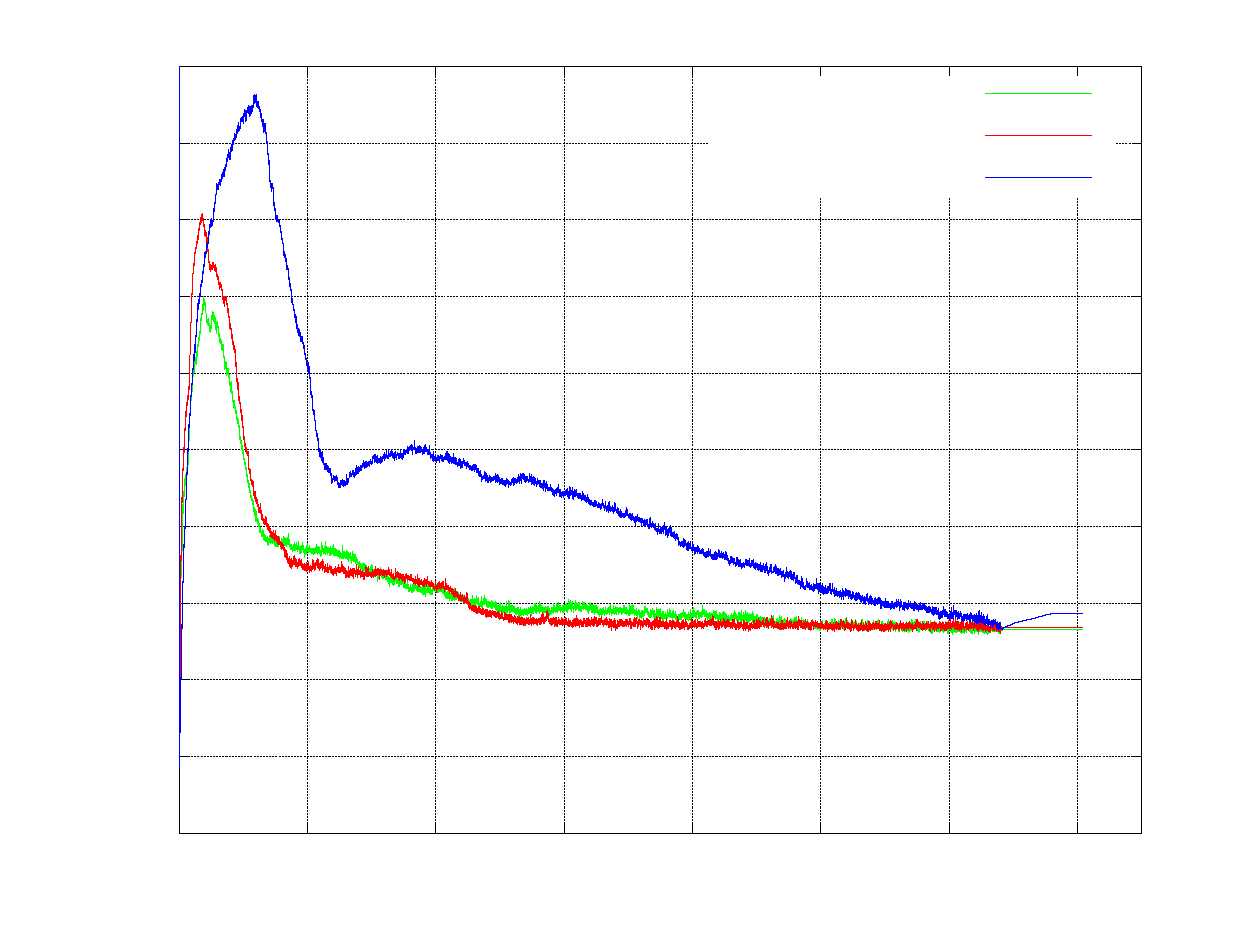
\includegraphics{./images/mlPosition7ThetaGA.eps}}%
    \gplfronttext
  \end{picture}%
\endgroup
}
  \put(-410,70){\rotatebox{90}{Μέσο ποσοστό κάλυψης κανόνων}}
  \put(-355,-20){\rotatebox{0}{Αριθμός δειγμάτων που έχουν παρουσιαστεί στον πληθυσμό}}
  \caption{Καμπύλες εξέλιξης του μέσου αριθμού κάλυψης δειγμάτων των κανόνων του πληθυσμού για τιμές $\theta_{exp}=\{4,20,40\}$ στο σύνολο δεδομένων $mlPosition7$.}
  \label{fig:mlPosition7ThetaGA}
\end{figure}


Μερικά πράγματα που μπορούμε να παρατηρήσουμε, είναι:
\begin{itemize}
\item Αύξηση του κατωφλίου εμπειρίας $\theta_{exp}$ σημαίνει πως θα περάσουν περισσότερες επαναλήψεις μέχρι το ΜαΣΤ να εμπιστευτεί έναν κανόνα και να του επιτρέψει να συμμετάσχει στην εξελικτική διαδικασία. Όπως είναι φυσικό, κανόνες που είναι γενικότεροι, καλύπτουν περισσότερα δείγματα του συνόλου δεδομένων, άρα συμμετέχουν σε περισσότερα Match Sets και, συνεπώς, η εμπειρία τους αυξάνεται με μεγαλύτερο ρυθμό από τους ειδικότερους από αυτούς κανόνες. Εφόσον οι κανόνες που σπάνε το φράγμα του $\theta_{exp}$ πρώτοι και συχνότερα είναι γενικοί, αυτό σημαίνει πως ο πληθυσμός των κανόνων οδηγείται από νωρίς σε αυξημένα επίπεδα γενίκευσης. Από μόνο του αυτό το γεγονός δεν είναι απαραίτητα ζημιογόνο, αλλά σε περιπτώσεις ανισοκατανομής των διακριτών συνδυασμών ετικετών ή/και επιλογής υπό-βέλτιστου συνδυασμού παραμέτρων $(\abs{I}, \theta_{GA}, maxPopulationSize, P_{\#A})$ είναι δυνατό ο Γενετικός Αλγόριθμος να μην μπορέσει να παράξει τους ειδικούς κανόνες εκείνους που θα καλύψουν τους διακριτούς συνδυασμούς ετικετών που εκπροσωπούνται από τα λιγότερα δείγματα στο σύνολο δεδομένων.

\item Όσο αυξάνει το κατώφλι $\theta_{exp}$, τόσο μετατοπίζεται αργότερα το σημείο στο οποίο ο πληθυσμός των κανόνων συναντά το ανώτατο του όριο, και άρα εκκινούν οι διαγραφές. Όσο γενικότερος ένας κανόνας, σε τόσα περισσότερα Correct Sets συμμετέχει, άρα τόσο περισσότερο κοντά στην τρέχουσα τιμή της χρονοσφραγίδας $timestamp$ του συστήματος θα βρίσκεται αυτή του κανόνα. Όταν οι κανόνες που καταφέρνουν αρχικά να ξεπεράσουν το κατώφλι είναι αναγκαστικά γενικότεροι, αυτό σημαίνει πως και τα περισσότερα Correct Sets θα πληρώνονται με κανόνες που καθιστούν μικρότερη τη διαφορά $timestamp - \overline{timestamp}([C_{l}])$, για δεδομένο $l$, και συνεπώς ο ρυθμός παραγωγής κανόνων καθίσταται μικρότερος από αυτόν για μικρότερες τιμές του κατωφλίου εμπειρίας $\theta_{exp}$.

\item Όπως φανερώνει η καμπύλη με μπλε χρώμα, όσο αυξάνει το κατώφλι $\theta_{exp}$, τόσο περισσότερο χρόνο χρειάζεται το ΜαΣΤ για να συγκλίνει προς τη βέλτιστη λύση. Αυτό σημαίνει πως αυξημένες τιμές του κατωφλίου, δυνητικά να χρειάζονται και μεγαλύτερο αριθμό επαναλήψεων εκπαίδευσης.

\item Αν παρατηρήσουμε το διάστημα ενημέρωσης, στο τελευταίο μέρος της εκπαίδευσης (για συνολική παρουσίαση περίπου $13 \cdot 10^{4}$ δειγμάτων), θα δούμε ότι το ΜαΣΤ, για $\theta_{exp}=40$, λόγω ίσως και της αργής του σύγκλισης, αποβάλλει τους κανόνες στο χαμηλότερο επίπεδο κάλυψης στα Match Sets (σε αντίθεση με τις προσεγγίσεις για $\theta_{exp}=\{4,20\}$ που τους έχουν αποβάλει ήδη), αυξάνοντας έτσι, εν τέλει, το μέσο ποσοστό κάλυψης των κανόνων του τελικού μοντέλου για το ίδιο πρόβλημα.
\end{itemize}


Οι παραπάνω παρατηρήσεις μας οδηγούν στα εξής συμπεράσματα: α) Ο ακριβής προσδιορισμός του κατωφλίου $\theta_{exp}$ θα πρέπει να γίνει σε σχέση με τις υπόλοιπες παραμέτρους του ΜαΣΤ, β) η διαδικασία προσδιορισμού του, ανάλογα με το σύνολο δεδομένων, είναι χρονοβόρα διότι και εδώ θα πρέπει να εφαρμόσουμε μια διαδικασία trial-and-error, γ) ίσως θα ήταν συμφερότερο να χρησιμοποιήσουμε δύο κατώφλια εμπειρίας, ένα για το διάστημα όπου η πληθικότητα του πληθυσμού είναι μόνιμα κάτω από το άνω όριό του και ένα για το διάστημα μετά την έναρξη των διαγραφών, αν και τότε θα έπρεπε να προσδιορίσουμε δύο κατώφλια αντί για ένα, και δ) ίσως θα έπρεπε να εγκαταλείψουμε εξ ολοκλήρου την προσέγγιση που θέτει ένα αυθαίρετο κατώφλι εμπειρίας και να βρούμε μία αντικειμενική συνθήκη για την έκπτωση της καταλληλότητας.


Μία τέτοια μεθοδολογία, όπως προσδιορίζεται από το τελευταίο συμπέρασμα, θα μπορούσε να βασίζεται στην αντικατάσταση του κατωφλίου εμπειρίας, και άρα της σχετικότητας του βαθμού γενίκευσης ενός κανόνα, από μία δυαδική σχέση που θα βασίζεται στο αν ο κανόνας έχει κληθεί να συμμετάσχει σε παραπάνω Match Sets από ότι είναι ο αριθμός των δειγμάτων του συνόλου δεδομένων, ή όχι. 

\begin{equation}
\label{eq:altFit}
fitness'(i) = \left\{
\begin{array}{ c l }
	\displaystyle 0, & D.checked = false
	\\
	\\
	\displaystyle \Big(\frac{tp(i)}{msa(i)}\Big)^{\nu}, & $αλλού$
\end{array}
\right.
\end{equation}


Με αυτό τον τρόπο, απομακρύνουμε τον προσδιορισμό ακόμα μίας παραμέτρου (δύο για την ακρίβεια, όπως θα φανεί παρακάτω) και θέτουμε ένα αντικειμενικό κριτήριο εμπιστοσύνης του συστήματος προς τους κανόνες. Ιδίως εάν το πρόβλημα διαθέτει μικρό αριθμό ετικετών, όμως, ίσως χρειαστούν περισσότερες επαναλήψεις για τη σύγκλιση σε κάποια βέλτιστη λύση, καθώς θα καθυστερείται η ανανέωση του πληθυσμού των κανόνων.


Τέλος, θα πρέπει να επισημάνουμε πως το κατώφλι $\theta_{exp}$ στη συνιστώσα εξερεύνησης και το κατώφλι $\theta_{del}$ στη λειτουργία διαγραφής είναι οι δύο όψεις του ίδιου νομίσματος και ο προσδιορισμός του ενός πρέπει να γίνει σε συσχέτιση με τον προσδιορισμό του άλλου. Εάν κρατήσουμε τη δομή της Εξ. \ref{eq:deletionFormula} (που αφορά στην ποσότητα $d(i)$ η οποία προσδιορίζει την πιθανότητα διαγραφής ενός κανόνα) και σταθερό το $\theta_{exp}$, ανεξάρτητα από τις ακριβείς πιθανότητες διαγραφής, η διαφορά 

\begin{equation}
\theta_{del}-\theta_{exp} > 0
\end{equation}
\\
θα προσδιορίσει το διάστημα χάριτος στο οποίο κανόνες θα έχουν τη δυνατότητα, ανάλογα με την καταλληλότητά τους, να αποτελέσουν υποψήφιους γονείς και να διαιωνίσουν τα γονίδιά τους, χωρίς να κινδυνεύουν να διαγραφούν πρόωρα σε αντίθετη περίπτωση.


\subsection{Διάστημα Ενημέρωσης}
Στο γράφημα του Σχήματος \ref{fig:enronZeroCoveragePrevention} παρατηρούμε την πτώση του αριθμού των κανόνων του πληθυσμού στις τελευταίες επαναλήψεις. Η διαδικασία εκπαίδευσης περιλαμβάνει δύο διαδοχικά στάδια: α) την εκπαίδευση του ΜαΣΤ, όπου κάθε δείγμα του συνόλου δεδομένων εισάγεται σε αυτό $\abs{I}$ φορές και στην οποία η λειτουργία του Γενετικού Αλγορίθμου είναι ενεργοποιημένη και β) το διάστημα ενημέρωσης, $u \cdot \abs{I}$ επαναλήψεων, με $u \in [0, 1]$, όπου η παραγωγή νέων κανόνων είναι απενεργοποιημένη (άρα και η λειτουργία διαγραφής κανόνων μέσω επιλογής ρουλέτας). 

Το διάστημα ενημέρωσης ενσωματώνεται στη διαδικασία εκπαίδευσης ώστε να παρέλθει αρκετός χρόνος, δηλαδή ικανός αριθμός επαναλήψεων, ώστε η πραγματική τιμή της καταλληλότητας των κανόνων και η καταλληλότητα μετά την έκπτωσή της που βασίζεται στην εμπειρία Εξ. \ref{eq:fitnessDiscount}, να ισούνται αριθμητικά. Γενικότερα, αυτό το διάστημα εξυπηρετεί στη σταθεροποίηση των παραμέτρων των κανόνων (όπως η εκτίμηση $cs$ ή, σημαντικότερα, η καταλληλότητά τους) που δημιουργήθηκαν στην τελευταία επανάληψη της διαδικασίας εκπαίδευσης. Σε κάθε περίπτωση, το διάστημα ενημέρωσης, ανεξάρτητα από το μήκος του, είναι αναπόσπαστο κομμάτι της διαδικασίας δημιουργίας του τελικού μοντέλου, ώστε η συνιστώσα επίδοσης να χρησιμοποιεί τις ακριβείς τιμές καταλληλότητας των κανόνων και να ταξινομήσει ορθά, με βάση το πλήρες σύνολο κανόνων που παρήγε το ΜαΣΤ. Αν η συνιστώσα επίδοσης ενός ΜαΣΤ κάνει και αυτή χρήση της έκπτωσης της καταλληλότητας με βάση την εμπειρία, θα πρέπει να ισχύει:

\begin{equation}
u \cdot \abs{I} > \theta_{exp}
\end{equation}
\\
Σε διαφορετική περίπτωση, αρκεί έστω και μία τελική επανάληψη με το Γενετικό Αλγόριθμο απενεργοποιημένο, ώστε οι κανόνες που δημιουργήθηκαν στην τελευταία επανάληψη να εξετάσουν για μία φορά το σύνολο δεδομένων και να σταθεροποιήσουν τις παραμέτρους τους.

Αν και η συνιστώσα επίδοσης του GMl-ASLCS χρησιμοποιεί απευθείας τις τιμές της ακρίβειας (και όχι της καταλληλότητας) των κανόνων για το συμπερασμό των ετικετών των δειγμάτων του συνόλου ελέγχου, εδώ χρησιμοποιούμε το διάστημα ενημέρωσης για να απομακρύνουμε από τον πληθυσμό κανόνες που πληρούν τις προϋποθέσεις αφαίρεσής τους από τον πληθυσμό, μέσω του μηχανισμού Διεύρυνσης της Μέσης Κάλυψης που περιγράφηκε στην Παρ. \ref{subsec:controlInM}. Η μείωση του αριθμού των κανόνων που παρατηρούμε στο γράφημα του Σχήματος \ref{fig:enronZeroCoveragePrevention} στις τελευταίες επαναλήψεις, οφείλεται ακριβώς στην εφαρμογή του μηχανισμού αυτού.

 


\subsection{Παρατηρήσεις πάνω στη μέση κάλυψη} 
\label{subsec:commentsOnCov}
Μία εικόνα για τον αριθμό δειγμάτων που καλύπτουν οι κανόνες του πληθυσμού λαμβάνουμε από το μέσο ποσοστό κάλυψης δειγμάτων των κανόνων, το οποίο παριστάνεται με κόκκινο χρώμα για το σύνολο δεδομένων $emotions$ στο γράφημα του Σχήματος \ref{fig:emotionsNsPlusCov}. Αυτό που παρατηρούμε είναι ότι το μέσο ποσοστό δειγμάτων που καλύπτουν οι κανόνες ακολουθεί τη μορφή της πορείας του μέσου αριθμού κανόνων των Corrects Sets: αυξάνει μέχρι ο πληθυσμός να φτάσει για πρώτη φορά το άνω όριό του και για το διάστημα που ακολουθεί, φθίνει, μέχρι το τέλος της εκπαίδευσης. Όσο πιο γενικός είναι ένας κανόνας, τόσα περισσότερα δείγματα καλύπτει, άρα συμμετέχει σε περισσότερα Match Sets και άρα σε περισσότερα Correct Sets. Στους γενικότερους κανόνες δίνονται περισσότερες ευκαιρίες αναπαραγωγής λόγω ακριβώς του γεγονότος ότι συμμετέχουν σε περισσότερα $[C]$ από ότι οι υπόλοιποι κανόνες, παράγοντας απογόνους που διατηρούν και διευρύνουν αυτή τη γενίκευση πάνω στα δείγματα. Αυτή η ροπή συμμετοχής σε περισσότερα $[C]$, προκαλεί την αύξηση του μεγέθους των Correct Sets. Όμως, το κυρίαρχο κριτήριο διαγραφής για έναν κανόνα είναι το μέγεθος των Correct Sets στα οποία αυτός συμμετέχει, το οποίο είναι και ικανή συνθήκη για να διαγραφεί, αλλά όχι αναγκαία. Ανάμεσα στους κανόνες που διαγράφονται, βρίσκονται και αυτοί που χαρακτηρίζονται από αυξημένη γενικότητα σε σχέση με τους υπόλοιπους. Για αυτό ακριβώς χρησιμοποιούμε και ως κριτήριο διαγραφής την καταλληλότητα, ώστε να διαχωρίσουμε τους κανόνες που είναι υπέρ-γενικοί και η προβλεπτική τους ικανότητα είναι χαμηλή, από τους κανόνες που καταφέρνουν να ισορροπήσουν ανάμεσα στην επαρκή γενικότητα και την ικανοποιητική καταλληλότητα\footnote{Εν γένει, αυτή η εργασία αποφεύγει τη χρήση απόλυτων όρων, καθώς, η λύση κάθε προβλήματος απαιτεί διαφορετικά επίπεδα γενικότητας ή/και καταλληλότητας των κανόνων.}.


Είναι εύκολο να παρατηρήσει κανείς, με βάση και το περιεχόμενο της παραπάνω παραγράφου, ότι μεγαλύτερα μεγέθη πληθυσμών, με σταθερό ρυθμό παραγωγής κανόνων $\theta_{GA}$ και αριθμό επαναλήψεων, θα είχαν ως αποτέλεσμα μεγαλύτερα επίπεδα τιμών μέσου μεγέθους των Correct Sets $\overline{cs}$ και μεγαλύτερα επίπεδα κάλυψης.

Πράγματι, θέτοντας το μέγιστο αριθμό μικρο-κανόνων που μπορεί να συγκρατήσει ο πληθυσμός σε μεγαλύτερες τιμές, το σημείο καμπής στο οποίο εκκινούν οι διαγραφές κανόνων μετατοπίζεται σε αργότερο χρόνο, όπου, εν γένει, τα διάφορα Correct Sets αποτελούνται από περισσότερους κανόνες και συνεπώς όπου το $\overline{cs}$ είναι αυξημένο, όπως και η μέση κάλυψη των τελικών κανόνων. Αυτή, βέβαια, δε δύναται να είναι συνεχώς αύξουσα: αν δεν ετίθετο όριο στο μέγεθος του πληθυσμού και των επαναλήψεων δε θα έφτανε στην τιμή $1$. 

Μικρότερη τιμή της παραμέτρου $\theta_{GA}$, για ίσο αριθμό μικρο-κανόνων, θα είχε ως αποτέλεσμα τη μετατόπιση του παραπάνω σημείου νωρίτερα, λόγω του μεγαλύτερου ρυθμού παραγωγής κανόνων και άρα της πιο γρήγορης άφιξης του πληθυσμού στο όριό του. Αν αυξάναμε τον αριθμό των επαναλήψεων, κρατώντας σταθερά το αριθμητικό όριο του πληθυσμού και το $\theta_{GA}$, θα παρατηρούσαμε μία συνεχή πτώση τόσο του μέσου μεγέθους των $[C]$, όσο και της μέσης κάλυψης των κανόνων. Η πτώση αυτή, επειδή είναι εκθετική, προκαλεί μείωση των παραπάνω μεγεθών με όλο και μικρότερο βαθμό, δηλαδή παρατηρείται μικρότερος ρυθμός πτώσης τους όσο αυξάνουν οι επαναλήψεις. 

Παράλληλα, ο ρυθμός γενίκευσης γνωρισμάτων $P_{\#A}$ είναι και αυτός ένας καθοριστικός παράγοντας στη διαδικασία εκπαίδευσης, καθορίζοντας άμεσα την ισορροπία ανάμεσα στη γενίκευση και την ακρίβεια του τελικού μοντέλου. Κάθε σύνολο δεδομένων απαιτεί και διαφορετικό $P_{\#A}$, ανάλογα με το βαθμό πληρότητας του, τον καθορισμό των παραπάνω τριών μεταβλητών και τη δυνατότητα των δειγμάτων του συνόλου δεδομένων να "ομαδοποιηθούν" στην αναπαράστασή τους από κανόνες, τόσο στο τμήμα συνθήκης όσο και στο τμήμα απόφασής τους.

Σε κάθε περίπτωση, η διαδικασία εύρεσης ενός αξιόπιστου συνόλου $$(\abs{I}, \theta_{GA}, maxPopulationSize, P_{\#A})$$ είναι επίπονη για κάθε σύνολο δεδομένων $D$, λόγω της εσωτερικής δομής του $D$ και της στοχαστικής φύσης των ΜαΣΤ. 

Εν γένει, η τιμή της παραμέτρου $\theta_{GA}$ θα πρέπει να καθορίζεται με γνώμονα τη μη βιαιότητα ανανέωσης κανόνων στο εσωτερικό του πληθυσμού. Μικρές τιμές της σημαίνει ότι ο ρυθμός παραγωγής κανόνων γίνεται μεγαλύτερος, συνεπώς και ότι ο ρυθμός διαγραφής κανόνων γίνεται μεγαλύτερος. Σε αυτό το πλαίσιο λειτουργίας, στο ζυγό της καταλληλότητας και της γενικότητας, η πλάστιγγα γέρνει υπέρ της καταλληλότητας για δύο λόγους. Πρώτον, χρειάζονται λιγότερες επαναλήψεις για την επίτευξη του ισοδύναμου μεγέθους μέσης κάλυψης λόγω της μεγαλύτερης παραγωγής και διαγραφής κανόνων και βάσει των παρατηρήσεων των δύο πρώτων παραγράφων αυτής της ενότητας και, δεύτερον, υπάρχει μεγαλύτερη πίεση για εύρεση γονέων πλέον κατάλληλων και, συνεπώς, λιγότερο γενικών. Αντίστροφα, μία μεγάλη τιμή του $\theta_{GA}$ δε θα παρείχε επαρκή πίεση προς την εύρεση κατάλληλων κανόνων, λόγω και της αραιότερης παραγωγής κανόνων, ενώ θα μετατόπιζε τον ορίζοντα διαγραφών αργότερα, έχοντας σαν αποτέλεσμα αυξημένη γενικότητα κανόνων, λόγω της αραιής παραγωγής και διαγραφής κανόνων, σε βάρος της εξέλιξης των κατάλληλων λύσεων. Εν κατακλείδι, η διαδικασία καθορισμού μίας λειτουργικής τετράδας παραμέτρων $(\abs{I}, \theta_{GA}, maxPopulationSize, P_{\#A})$ δεν μπορεί να ιδωθεί ως μία αρθρωτή διαδικασία, ξεχωριστή για την καθεμία, αλλά ως ένα συνεργατικό έργο.


\subsection{Για το ρυθμό μεταβολής του μεγέθους του πληθυσμού στα πρώιμα στάδια της εκπαίδευσης}
Στα Σχήματα \ref{fig:enronFluctuations} και \ref{fig:enronZeroCoveragePrevention}, παρατηρούμε την απότομη άνοδο του αριθμού των μικρο-κανόνων του πληθυσμού μετά την είσοδο περίπου $5 \cdot 10^{4}$ δειγμάτων στο ΜαΣΤ. Μέχρι αυτό το κρίσιμο σημείο, το ΜαΣΤ έχει παράξει έναν περιορισμένο αριθμό κανόνων μέσω της λειτουργίας κάλυψης, ενώ η πλειοψηφία των κανόνων έχει δημιουργηθεί μέσω του Γενετικού Αλγορίθμου. Ωστόσο, λόγω του σχετικά μεγάλου αριθμού ετικετών του προβλήματος enron, με $\abs{L}=53$, και της χαμηλής τιμής της τρέχουσας χρονοσφραγίδας, η κατανομή των κανόνων ανά $[C]$ είναι τέτοια που ο μέσος όρος των χρονοσφραγίδων των κανόνων ξεπερνά το κατώφλι $timestamp([C]) - \theta_{GA}$ για μικρό αριθμό από Correct Sets. Υπενθυμίζουμε πως για να ενεργοποιηθεί η διαδικασία παραγωγής κανόνων μέσω του Γενετικού Αλγορίθμου, θα πρέπει
\begin{equation}
timestamp - \overline{timestamp}([C]) > \theta_{GA}
\end{equation}
\\
όπου $timestamp$ η τρέχουσα τιμής χρονοσφραγίδας τους συστήματος, 
\\
$\overline{timestamp}([C])$ ο μέσος όρος των χρονοσφραγίδων δημιουργίας των κανόνων ενός Correct Set και $\theta_{GA}$ το κατώφλι χρόνου. 

Το κατώφλι αυτό βλέπουμε ότι ξεπερνιέται όταν περάσει χρονικό διάστημα τέτοιο ώστε να υπάρχει ποικιλότητα ως προς το χρόνο δημιουργίας των κανόνων. Η ποικιλότητα αυτή μειώνει το μέσο όρο των χρονοσφραγίδων δημιουργίας των κανόνων στα $[C]$, σε σχέση με τη διαφορά $timestamp([C]) - \theta_{GA}$.


\section{Αρθρωτές Τροποποιήσεις}
\label{sec:alterations}
Μέχρις αυτού του σημείου, έχουμε περιγράψει πλήρως τις βασικές λειτουργίες του GMl-ASLCS και τα σημεία διαφοροποίησης του από τον GMl-ASLCS$_{\:0}$. Σε αυτή την ενότητα θα εξετάσουμε μερικά περαιτέρω σημεία στα οποία θα μπορούσαμε να διαφοροποιήσουμε τη λειτουργία του GMl-ASLCS, αλλά δεν περιλαμβάνονται στο βασικό ορισμό του. Τα σημεία αυτά θα μελετηθούν στη συνέχεια σε σχέση με αυτόν.





\subsection{Τροποποίηση της Ενημέρωσης Καταλληλότητας στη Συνιστώσα Ενίσχυσης}
\label{subsec:qfitness}
Όπως περιγράφηκε στη γραμμή $7$ του Αλγ. \ref{alg:gmlaslcsUpdateFitness}, ο GMl-ASLCS υπολογίζει την καταλληλότητα ενός κανόνα απευθείας από το λόγο ορθών κατηγοριοποιήσεων προς τις συνολικές του κατηγοριοποιήσεις, υψωμένο σε μία δύναμη $\nu$. Σαφέστατα, είναι δυνατόν να υπάρξουν ποικίλοι τρόποι υπολογισμού της καταλληλότητας ενός κανόνα, αλλά σε αυτή την εργασία εξετάζουμε μόνο άλλη μία. Αυτή βασίζεται στην τεχνική \emph{Q-learning} \cite{WilsonZCS} που χρησιμοποιείται κατά κόρον στην ενισχυτική μάθηση και προσομοιάζει περισσότερο στο διαμοιρασμό καταλληλότητας που χρησιμοποιεί ο UCS. Έτσι, για δεδομένο κανόνα $rule$, αν $t$ και $t-1$ διακριτές διαδοχικές χρονικές στιγμές στις οποίες ενημερώνεται η καταλληλότητα του $rule$, $rule.tp$, ο αριθμός των ορθών και $rule.msa$ συνολικών κατηγοριοποιήσεών του, και $\beta$ ο ρυθμός μάθησης, η καταλληλότητα του $rule$ ενημερώνεται ως εξής:

\begin{equation}
fitness(rule,t) = fitness(rule, t-1) + \beta \cdot \left(\left(\frac{rule.tp}{rule.msa}\right)^{\nu} - fitness(rule, t-1)\right)
\end{equation}

\subsection{Τροποποίηση της Λειτουργίας Διαγραφής}
\label{subsec:ucsDeletion}
Αν και κάθε σύνολο δεδομένων έχει διαφορετικές ανάγκες ως προς τη διαγραφή κανόνων, το Σχήμα διαγραφής ενός ΜαΣΤ θα πρέπει να ενσωματώνει μία μέθοδο διαγραφής που να μπορεί να είναι εύρωστη για διαφορετικά σύνολα δεδομένων. Εφόσον η μέθοδος διαγραφής του UCS (Εξ. \ref{eq:aslcsDeletion}) αποδεικνύεται αξιόπιστη για προβλήματα μονοκατηγορικής ταξινόμησης και δεδομένης της ανάγκης μας για καλύτερο διαχωρισμό των υπό διαγραφή κανόνων μέσω της ανάθεσης πιθανοτήτων διαγραφής που βασίζονται στην ύψωση του αριθμού Euler στις παραμέτρους που αποτελούν τα κριτήρια διαγραφής, μπορούμε να ενσωματώσουμε τη μέθοδο διαγραφής του UCS στο πλαίσιο διαγραφής του GMl-ASLCS, αντικαθιστώντας την Εξ. \ref{eq:deletionFormula} στον υπολογισμό της πιθανότητας διαγραφής $P(i)$ ενός κανόνα $i$, με την:

\begin{equation}
\label{eq:aslcsDeletion}
d(i) = \left\{
\begin{array}{ c l }
\displaystyle e^{\frac{\displaystyle cs(i) \cdot F_{P}}{\displaystyle F_{micro}(i)}}, & experience(i) > \theta_{del} $ και $F_{micro}(i) < \delta \cdot F_{P}
\\
\\

\displaystyle e^{\displaystyle cs(i)}, & $αλλού$
\end{array}
\right.
\end{equation}


\subsection{Εναλλακτικές τιμές των μεταβλητών $\omega, \phi$}
\label{subsec:phiomega}
Όπως είδαμε στην Παρ. \ref{subsec:gmlaslcs0update}, οι μεταβλητές $\omega, \phi$ καθορίζουν το ποσό μεταβολής της ακρίβειας ενός κανόνα για κάθε ετικέτα για την οποία αδιαφορεί. Ο GMl-ASLCS ακολουθεί μία ασφαλή προσέγγιση, χρησιμοποιώντας ως $(\omega. \phi) \equiv (0.9, 1)$, ωστόσο, αυτό δεν είναι το μοναδικό ζευγάρι παραμέτρων το οποίο θα οδηγούσε στην ορθή αξιολόγηση κανόνων που περιλαμβάνουν αδιαφορίες στο τμήμα απόφασής τους. Ένα δεύτερο ζεύγος τιμών για τις παραμέτρους $\omega, \phi$, με το οποίο πειραματιστήκαμε είναι το $(\omega. \phi) \equiv (0, 0)$. Με αυτό τον τρόπο παραβλέπονται οι αδιαφορίες των κανόνων για ετικέτες και ο υπολογισμός της καταλληλότητάς τους βασίζεται μόνο στις σαφείς αποφάσεις που λαμβάνουν, υπέρ ή κατά αυτών. Σε συνδυασμό με τον αποκλεισμό των κανόνων που αδιαφορούν για μία δεδομένη ετικέτα $l$ από το να συμμετέχουν στο αντίστοιχο $[C_{l}]$ και χαμηλές τιμές πιθανότητας γενίκευσης ετικετών από το τμήμα κάλυψης, $P_{\#L} < 0.1$, αυτή η μέθοδος ενημέρωσης της καταλληλότητας των κανόνων φαίνεται ότι αποτελεί μία ορθή και αξιόπιστη εναλλακτική προσέγγιση στο ζήτημα του προσδιορισμού των δύο αυτών παραμέτρων (βλ. πειραματικά αποτελέσματα στην Παρ. \ref{subsec:resComm}). 


\subsection{Αρχικοποίηση Πληθυσμού μέσω Ομαδοποίησης}
\label{subsec:gmlaslcsClustering}
Η λειτουργία της κάλυψης, στα πλαίσια ορισμού των ΜαΣΤ, δημιουργεί κανόνες ταξινόμησης ως γενικευμένες εκδόσεις των δειγμάτων του συνόλου εκπαίδευσης $D$ στις περιπτώσεις που το ΜαΣΤ δε διαθέτει κάποιον κανόνα που να ενεργοποιείται για ένα δεδομένο παρεχόμενο δείγμα του $D$. Ο τελεστής κάλυψης συμπληρώνει το σύνολο κανόνων προοδευτικά και \emph{κατά τη διάρκεια} της εκπαίδευσης, δηλαδή σε στενή αλληλεπίδραση με τις διαδικασίες εξελικτικής αναζήτησης και διαγραφής που χρησιμοποιούνται από τα ΜαΣΤ. Στο \cite{tzima12}, γίνεται η πρώτη αναφορά σε αρχικοποίηση του πληθυσμού κανόνων \emph{πριν τη διαδικασία εκπαίδευσης}, για ΜαΣΤ μονοκατηγορικής ταξινόμησης. Η \emph{βασισμένη στην Ομαδοποίηση Αρχικοποίηση} εφαρμόζεται πριν την εκπαίδευση και συμπληρώνει τον τελεστή κάλυψης, έχοντας ως στόχο την παροχή ικανών αρχικών λύσεων για την εξελικτική συνιστώσα ανακάλυψης κανόνων. 

Εν γένει, η μέθοδος αρχικοποίησης μέσω ομαδοποίησης προσπαθεί να εκμεταλλευτεί τις δυνατότητες των αλγορίθμων ομαδοποίησης (clustering) για να παράξει ένα μη-τυχαίο σύνολο κανόνων το οποίο μπορεί να βοηθήσει την εξελικτική διαδικασία, προσδιορίζοντας τη “βάση" των κανόνων που εξελίσσει, ώστε το ΜαΣΤ να εστιάσει αποτελεσματικά στα βέλτιστα σημεία του χώρου αναζήτησης (στο βέλτιστο σύνολο κανόνων για το υπό μελέτη πρόβλημα κατηγοριοποίησης). Διαισθητικά, αυτό το μη-τυχαίο σύνολο αρχικών κανόνων θα πρέπει να βασίζεται στη διαθέσιμη πληροφορία για το πρόβλημα και να παρέχει μία περιεκτική περίληψη της γνώσης που περιέχεται σε αυτό. Στόχος είναι η βελτίωση συνολικά της προβλεπτικής ικανότητας των ΜαΣΤ και η ερμηνευσιμότητα των παραγόμενων μοντέλων.

Η μέθοδος επιλέγει ένα αντιπροσωπευτικό σύνολο σημείων - τα κεντροειδή - από το $D$ και τα μετασχηματίζει σε κανόνες κατάλληλους για την αρχικοποίηση του πληθυσμού του ΜαΣΤ, μέσω της παρακάτω διαδικασίας:

\begin{enumerate}
\item Το σύνολο εκπαίδευσης $D$ διαμερίζεται σε \emph{N} υποσύνολα, όπου \emph{N} είναι ο αριθμός των διακριτών συνδυασμών τιμών των ετικετών των δειγμάτων του $D$. Κάθε υποσύνολο $Partition_{i}$, $1 \leq i \leq N$, περιλαμβάνει όλα τα δείγματα του διακριτού συνδυασμού τιμών των ετικετών $i$ του $D$: 
\begin{equation}
\sum\limits_{i=1}^N Partition_{i} = D
\end{equation}
\item Για κάθε $Partition_{i}$:

	\begin{enumerate}
	\item Τα δείγματά του ομαδοποιούνται σε $M_{i} = \left\lceil\gamma \cdot \abs{Partition_{i}}\right\rceil$ συστάδες, όπου $\abs{Partition_{i}}$ είναι ο αριθμός δειγμάτων του $Partition_{i}$ και $\gamma \leq 1$ μία οριζόμενη από το χρήστη παράμετρος.
	\item Για κάθε συστάδα $cluster_{j}$, $1\leq j \leq M_{i}$ που αναγνωρίστηκε στο βήμα (2α'), βρίσκεται το κεντροειδές της μέσω του αλγορίθμου k-means και βάσει των γνωρισμάτων του δημιουργείται ένας κανόνας του οποίου το τμήμα συνθήκης αποτελεί, εν γένει, μία γενίκευσή του, ανά γνώρισμα, όπως και στην περίπτωση εφαρμογής του τελεστή κάλυψης. Το τμήμα απόφασης του κανόνα τίθεται ίδιο με το διακριτό συνδυασμό τιμών ετικετών που συσχετίζεται με το $Partition_{i}$.
 	\end{enumerate}
	\item Όλοι οι $$K = \sum\limits_{i=1}^N \sum\limits_{j=1}^{\abs{M_{i}}}rule_{ij}$$ κανόνες της μορφής
	\\
	 $$rule_{ij}: \: ruleCondition_{ij} \rightarrow distinctLabelCombination_{i}$$ που δημιουργήθηκαν από την ομαδοποίηση του συνόλου εκπαίδευσης, συγχωνεύονται για να δημιουργήσουν το σύνολο κανόνων που θα χρησιμοποιηθεί για την αρχικοποίηση της εκπαιδευτικής διαδικασίας.
\end{enumerate}

\section{Σύνοψη}
Τα βασικά σημεία που παρουσιάστηκαν σε αυτό το κεφάλαιο συνοψίζονται παρακάτω.

\begin{enumerate}[I]
\item Παρουσιάσαμε τους λόγους για την επινόηση του τελεστή Διασταύρωσης Δύο Τμημάτων που προσιδιάζει περισσότερο στη φύση των προβλημάτων πολυκατηγορικής ταξινόμησης και που αποφεύγει την εναλλαγή διαφορετικών ετικετών από αυτή για την οποία σχηματίστηκε το Correct Set στο οποίο εφαρμόζεται η λειτουργία του Γενετικού Αλγορίθμου (Παρ. \ref{subsec:gmlaslcsCrossover}).

\item Εκθέσαμε τα προβλήματα που επιφέρει η συγκράτηση κανόνων μηδενικής κάλυψης στον πληθυσμό κανόνων των ΜαΣΤ και προτείναμε μία μέθοδο μη εισαγωγής τους στον πληθυσμό, που είναι ανεξάρτητη από τον αριθμό των ετικετών του προβλήματος και συνεπώς μπορεί να εφαρμοστεί ακόμα και σε μονοκατηγορικά ΜαΣΤ (Παρ. \ref{subsec:gmlaslcsZeroCov}).

\item Περιγράψαμε την ανανεωμένη διαδικασία εισαγωγής απογόνων στον πληθυσμό κανόνων (Παρ. \ref{subsec:subsumptionAndInsertion}) μετά τον έλεγχό τους για υπαγωγή (Παρ. \ref{subsec:subsumptionAndInsertion}).

\item Εισήγαμε μία νέα μέθοδο διαγραφής κανόνων, εξηγήσαμε γιατί είναι προτιμότερο να μην χρησιμοποιείται η προσέγγιση του μεγέθους των Correct Sets στα οποία συμμετέχει ένας κανόνας στα πρώτα του βήματα μέσα στον κύκλο εκπαίδευσης των ΜαΣΤ όσον αφορά στη διαγραφή του και τους λόγους χρήσης του αριθμού Euler ως βάση για την ύψωση σε αυτή των κριτηρίων διαγραφής (Παρ. \ref{subsec:gmlaslcsDeletion}).

\item Διαπιστώσαμε το χαμηλό επίπεδο μέσης κάλυψης των κανόνων του τελικού μοντέλου του GMl-ASLCS$_{\:0}$ και προτείναμε την εφαρμογή μίας πρωτότυπης μεθόδου για την αύξησή του (που και αυτή είναι ανεξάρτητη του αριθμού των ετικετών του προβλήματος και συνεπώς μπορεί να βρει εφαρμογή και σε προβλήματα απλής ταξινόμησης), κάνοντας την υπόθεση πως για δεδομένο δείγμα εκπαίδευσης είναι δυνατόν να βρούμε τους συσχετισμούς εκείνους που θα μας επιτρέψουν να αφαιρέσουμε κανόνες που στην ουσία αποτελούν πλεονασμό πληροφορίας (Παρ. \ref{subsec:controlInM}).

\item Σχολιάσαμε τη λειτουργία ορισμένων αρθρωτών τμημάτων των ΜαΣΤ και προτείναμε περαιτέρω τροποποίησής τους, βάσει των παραπάνω σχολίων, προς κατευθύνσεις που θα μπορούσαν να εξερευνηθούν και να επεκταθούν στο μέλλον (εν. \ref{sec:alterations}).

\end{enumerate}
 





